\documentclass[conference]{IEEEtran}
\IEEEoverridecommandlockouts
\usepackage{cite}
\usepackage{amsmath,amssymb,amsfonts}
\usepackage{graphicx}
\usepackage{booktabs}
\usepackage{multirow}
\usepackage{makecell}
\usepackage{xcolor}
\usepackage{url}
\usepackage{tikz}
\usetikzlibrary{positioning,arrows.meta,shapes.geometric,fit,calc}
\usepackage{pgfplots}
\pgfplotsset{compat=1.17}
\usepgfplotslibrary{groupplots}

\begin{document}

% Original title: Attributing Security in a Local, Zero-Cost Defense-in-Depth Pipeline for Retrieval-Augmented Generation
\title{Attributing Security in a Local, Zero-Cost Defense-in-Depth Pipeline for Retrieval-Augmented Generation: Instruction Injection Is Contained, Knowledge Corruption Is Not}

\author{\IEEEauthorblockN{Anonymous Authors}}

\maketitle

\begin{abstract}
Retrieval-Augmented Generation (RAG) lets an attacker place either \emph{instructions} or \emph{false facts} in the context window through retrieved passages. Deployed systems stack imperfect defenses but rarely measure which layer provides the protection. We build a thirteen-stage, fully local, zero-cost defense pipeline and attribute its security stage by stage on 920 evaluation rows across seven sets and two scoring protocols, including independent PoisonedRAG, BIPIA, and deepset data, with paired tests within each set. Our central finding is a scope boundary. The pipeline contains instruction-carrying injection, but it offers no measurable protection against knowledge corruption. First, on instruction-carrying attacks, no canary leaked into any delivered answer (0 of 132 delivered) and every poisoned chunk was redacted before generation (74/74), attack success on delivered outputs falls from 29.5\% to 3.5\% under the seven-layer single-generator stack ($n=200$, $p<10^{-13}$), and 45/50 BIPIA attacks are blocked (0/50 undefended). On the same 200 attacks, the seven-layer single-generator stack outperforms an LLM-Guard firewall and Spotlighting (3.5\% vs.\ 21.0\% and 23.0\% ASR, $p<10^{-7}$), matches the ControlNET detector used as a firewall (4.5\%, $p=0.77$), and outperforms an adapted implementation of the Sentinel--Strategist orchestrator ADO (28.5\%, $p<10^{-11}$). Second, a single-generator ablation with a fully crossed factorial shows that three layers (per-chunk sanitization, grounding, and refusal on detection) act as near-independent filters and come within 2.4 points of the seven-layer stack on these instruction-bearing attacks (4.7\% vs.\ 4.2\% at $n=424$, 95\% upper bound of the difference 2.4 points); on assertion-only attacks the same three layers are significantly worse than seven (62.5\% vs.\ 35.0\%, $p=0.003$, $n=40$), and protection varies with attacker wording. Third, a co-activation detector designed for conjunctive sub-threshold attacks never fires validly on saturated classifier scores, and we prove that this is structural. Reading graded logit margins instead recovers 24/30 valid fires at 1/80 benign false fires (6/200 on held-out benign questions), but only 8/30 on external BIPIA data. Fourth, knowledge corruption is out of reach of this defense class: on PoisonedRAG the defended pipeline is no better than undefended RAG (90.7\% vs.\ 91.3\%, $p=1.0$), because every effective layer keys on instruction signatures that fluent false passages lack. The full stack runs on an 8~GB laptop GPU at a median of 15.3~s per query, or 8.6~s with its encoders moved to the GPU in fp16.
\end{abstract}

\begin{IEEEkeywords}
Retrieval-augmented generation, prompt injection, LLM security, defense in depth, indirect injection, local inference, guardrail models.
\end{IEEEkeywords}

\section{Introduction}
Large language models (LLMs) are now embedded in systems that read e-mail, browse the web, and query proprietary databases. Retrieval-Augmented Generation (RAG) supports such knowledge-intensive tasks by conditioning the model on passages retrieved at query time rather than on parametric memory alone~\cite{lewis2020rag}, and it has become the standard architecture for enterprise question answering, programming assistants, and chatbots. This architecture also creates an attack surface that a closed model does not have: every retrieved passage is an untrusted input channel. An attacker who can influence retrievable content, for example by editing a wiki page, posting a review, or poisoning a data source, can deliver instructions or false facts into the context window without any involvement of the end user. Greshake et al.\ first demonstrated this \emph{indirect prompt injection} against production applications~\cite{greshake2023}, and prompt injection now heads the OWASP Top~10 for LLM applications~\cite{owasp2025}. Most available defenses assume paid cloud services such as moderation APIs, hosted judges, and managed vector stores. Routing every prompt and retrieved document through a third-party classifier, however, exposes the very data that a private RAG deployment is meant to protect. We therefore require every component to run locally on commodity hardware, under an open-weight or permissive licence, at no licence or API cost.

Real deployments stack several imperfect defensive layers rather than relying on one. When such a pipeline stops an attack, however, it is rarely clear which layer was responsible: whether a new detector adds anything over the earlier layers, or whether those layers would have stopped the attack without it. This paper addresses that attribution question.

\textbf{Scope.} We distinguish two attacker goals that share the same retrieval channel. In \emph{instruction injection} (direct, indirect, and conjunctive), the payload tries to make the model follow attacker instructions. In \emph{knowledge corruption}~\cite{zou2025poisonedrag}, a fluent passage asserts a false fact and contains no instruction at all. Our pipeline is designed for, and claims protection against, the first. We evaluate the second deliberately, to locate the boundary of what this defense class can do. On PoisonedRAG it provides no measurable protection. We therefore present knowledge corruption as an open problem that requires different mechanisms, such as provenance and corroboration, not as a threat our system mitigates.

Our contributions are as follows. (C1) A zero-cost, fully local thirteen-stage pipeline built from known components, in which the input gate's risk score is propagated to downstream stages (Section~\ref{sec:method}); we do not claim a new detector. (C2) A paired attribution protocol for layered RAG defenses: leave-one-out, single-layer, and a fully crossed three-layer factorial on identical rows, exact paired tests, an independence null for interactions, a measured run-to-run noise floor, and class-conditional repetition. It applies standard ablation and factorial designs~\cite{fawcett2016ablation,hutter2014fanova} and is released with frozen per-row outputs and a claim-by-claim checker. (C3) Findings that an end-to-end comparison hides, for the seven-layer single-generator configuration: sanitization, grounding, and refusal act as near-independent filters with comparable shares; on instruction-bearing attacks they come within 2.4 points of all seven layers; on assertion-only attacks they do not, because the guarded prompt, harmful on its own against instruction-bearing attacks, carries that defense; and the measured protection depends on attacker wording (Section~\ref{sec:ablation}). (C4) A closed-form argument that a co-activation detector on saturated classifier scores cannot fire on its target band, with a graded-margin repair (Section~\ref{sec:negative}), and a stage-by-stage account of why this defense class does not reduce PoisonedRAG knowledge corruption (Sections~\ref{sec:external} and~\ref{sec:semantic}).

The study pursues four objectives.
\begin{enumerate}
\item[(i)] \textbf{Local, Zero-Cost Pipeline:} Create a RAG pipeline with layers of defense made only from open-source and free-of-charge components.
\item[(ii)] \textbf{Security Attribution:} Use paired statistics to attribute security results to each stage of the pipeline, rather than reporting accuracy metrics for each detector.
\item[(iii)] \textbf{Conjunctive Detection Feasibility:} Evaluate the ability of the signature detector to recognize synthetic multi-channel attacks using experimental data and theoretical reasoning.
\item[(iv)] \textbf{Scope the Residual Gap:} Identify attack types that may still bypass the pipeline and investigate the reasons for their non-detection.
\end{enumerate}

\section{Related Work}
\textbf{Adaptive RAG.} Self-RAG trains a model to emit reflection tokens that decide when to retrieve and when to critique~\cite{asai2024selfrag}; Corrective RAG adds an evaluator that scores retrieval quality~\cite{yan2024crag}; and FLARE retrieves again when generation confidence is low~\cite{jiang2023flare}. Each turns a single forward pass into an iterative process in which a late signal revises an earlier decision. Our closed-loop controller adopts this structure but controls security risk instead of answer quality.

\textbf{Prompt-injection attacks.} Perez and Ribeiro showed that hand-crafted prompts such as ``ignore previous instructions'' hijack GPT-3~\cite{perez2022}; Greshake et al.\ extended the threat to indirect injection through retrieved content~\cite{greshake2023}; Liu et al.\ formalized prompt injection as an optimization problem and benchmarked defenses~\cite{liu2024formalizing}; and Zou et al.\ showed that adversarial suffixes transfer across models~\cite{zou2023}. PoisonedRAG~\cite{zou2025poisonedrag} corrupts the knowledge base with fluent false passages, and BIPIA~\cite{yi2023bipia} benchmarks indirect injection; we use both as external test sets.

\textbf{Detectors and structural defenses.} The fine-tuned DeBERTa-v3 injection classifier~\cite{he2021debertav3,protectai2024} gives a fast injection score on CPU, and Llama Guard gives a categorical safety verdict~\cite{inan2023llamaguard}. They fail differently: the injection classifier flags harmless instruction-like text and misses role-play framing, while the safety classifier handles framing but misses syntactic injection. Combining them at the input gate is therefore reasonable. Spotlighting wraps retrieved context in delimiters so the model treats it as data rather than instructions, cutting attack success on GPT models from over 50\% to under 2\%~\cite{hines2024spotlighting}. The dual-LLM pattern~\cite{willison2023dual} and CaMeL~\cite{debenedetti2025camel} separate privileged control from untrusted data, so their security does not depend on any classifier detecting the attack. Reference-free grounding metrics such as RAGAS decompose an answer into claims and verify each against the context~\cite{es2023ragas}, and disagreement between models, measured with Sentence-BERT embeddings~\cite{reimers2019sbert}, can serve as an additional risk signal.

\textbf{Defense systems for RAG.} Closest to our setting are three recent systems. ControlNET~\cite{yao2025controlnet} detects malicious RAG queries from shifts in LLM activations; the Sentinel--Strategist orchestrator (ADO)~\cite{palleria2026ado} uses LLM controllers to switch among defenses such as TrustRAG and DP-RAG; and Saleem et al.~\cite{saleem2026layered} combine an input classifier, a provenance-based instruction hierarchy, and an output auditor, targeting GPT-4o through its API as well as local Llama~3 and Mistral models. Saleem et al.\ come closest to stage-level attribution: they evaluate all seven subsets of their three layers. Like ControlNET and ADO, however, they report point estimates without confidence intervals or significance tests. We did not find among these works one that compares configurations with paired tests on identical rows or reports a component of its own system that fails to contribute. Per-component ablations of layered prompt-injection defenses also appear in Ramakrishnan and Balaji~\cite{ramakrishnan2025securing} and in LlamaFirewall~\cite{chennabasappa2025llamafirewall}. Defenses designed for knowledge corruption take a different route: RobustRAG answers from each retrieved passage separately and aggregates with certified guarantees~\cite{xiang2024robustrag}, and TriShieldRAG combines ingest screening, trust-weighted re-ranking, and cross-model consensus, reporting a large reduction on non-adaptive PoisonedRAG and little against an adaptive attacker~\cite{trishield2026}. Our attribution design follows classical ablation and functional-ANOVA analyses of configurations~\cite{fawcett2016ablation,hutter2014fanova}.

\textbf{Distinction from prior work.} Most individual components we use are not new: the classifiers~\cite{protectai2024,inan2023llamaguard}, spotlighting~\cite{hines2024spotlighting}, canary tokens, and grounding checks~\cite{es2023ragas} are all known. We do not claim a new detector. Our contribution is the careful application of established attribution designs to a layered RAG defense, and the findings it yields (contributions C1--C4 in the Introduction; Table~\ref{tab:positioning}). The forward-propagated risk score and fail-closed controller are tested rather than asserted, and add no measured security. The practical result is that, on instruction-bearing attacks, a three-layer subset of the cascade comes within 2.4 points of the full stack (Section~\ref{sec:ablation}), while on assertion-only attacks it does not; the paper therefore argues for a simpler configuration chosen per threat, not a more complex one.

\begin{table}[t]
\centering
\caption{Positioning against related RAG and prompt-injection defenses. \checkmark{} = provided; -- = not reported.}
\label{tab:positioning}
\setlength{\tabcolsep}{2.6pt}
\begin{tabular}{lccccc}
\toprule
Work & \makecell{Fully\\local} & \makecell{Context\\defense} & \makecell{Stage-level\\attribution} & \makecell{Paired\\tests} & \makecell{Negative\\results} \\
\midrule
Spotlighting~\cite{hines2024spotlighting} & -- & \checkmark & -- & -- & -- \\
CaMeL~\cite{debenedetti2025camel} & -- & \checkmark & -- & -- & -- \\
ControlNET~\cite{yao2025controlnet} & \checkmark & \checkmark & -- & -- & -- \\
ADO~\cite{palleria2026ado} & \checkmark & \checkmark & -- & -- & -- \\
Layered~\cite{saleem2026layered} & partial$^a$ & \checkmark & subsets$^b$ & -- & -- \\
\textbf{This work} & \checkmark & \checkmark & \checkmark & \checkmark & \checkmark \\
\bottomrule
\multicolumn{6}{l}{\footnotesize $^a$GPT-4o target and judge via API; others local.} \\
\multicolumn{6}{l}{\footnotesize $^b$All seven layer subsets; point estimates, no tests or CIs.} \\
\end{tabular}
\end{table}

Three gaps motivate the study. First, defense-in-depth RAG pipelines have not been evaluated with stage-level attribution, so it is unclear which layer produces the observed security effect; we address this with paired ablations (Section~\ref{sec:ablation}). Second, conjunctive sub-threshold multi-vector attacks are a recognized risk, but it is unclear whether a detector built on injection-signature channels can recognize them in theory or in practice; we examine this with a closed-form argument and empirical tests (Section~\ref{sec:negative}). Third, no evaluated answer-side signal reliably separates signature-free semantic misinformation from benign traffic; we measure this residual gap in Sections~\ref{sec:external} and~\ref{sec:semantic}.

\section{Proposed Method}\label{sec:method}
The system wraps a conventional RAG core (embed $\rightarrow$ retrieve $\rightarrow$ rerank $\rightarrow$ generate $\rightarrow$ ground) in a thirteen-stage defensive cascade (Table~\ref{tab:stages}). Its organizing idea is a risk score that propagates forward. A borderline prompt is not merely logged at the input gate. Its fused risk score tightens context sanitization, reranking, and grounding for that same request. A clean prompt therefore pays almost nothing, a borderline prompt pays for stricter downstream checks, and an obviously hostile prompt is rejected at the gate before retrieval and generation are spent on it. The pipeline adapts its strictness while keeping a fixed set of stages.

\subsection{Forward Cascade}
Stage~2 normalizes every prompt, removing zero-width characters, homoglyphs, and encoding tricks (NFKC, \texttt{ftfy}, base64 decoding). The normalized prompt enters the fusion input gate (Stage~3/3c), which combines the DeBERTa-v3 injection score with the categorical Llama Guard~3 verdict into a continuous risk score $r_{\text{fusion}}$ and a three-way decision (allow, review, block). The same $r_{\text{fusion}}$ is passed to Stages~6, 7, and 10 of the request. After embedding and vector search (Stages~4--5), Stage~6 scans each retrieved chunk separately for embedded instructions and redacts flagged chunks. Its threshold drops from 0.50 to 0.30 when $r_{\text{fusion}}>0.45$. Stage~6 also inserts a unique canary token into the context. The canary has no legitimate reason to appear in an answer, so its presence in the output (checked at Stage~10) shows that the model treated the context as instructions rather than data. Stage~7 reranks the surviving chunks with a cross-encoder. Stage~8 assembles a spotlighted prompt that forbids following instructions found in the context. Stage~9 sends the prompt to three local generators of different architectures, and their mutual disagreement (Sentence-BERT distance) is a further risk signal. Stage~10 checks that the answer is grounded in the context and rechecks the canary. Finally, an output rail masks PII with Presidio (Stage~11) and applies a DLP scanner (Stage~12). Stage~13 returns either the grounded answer or a fixed refusal with an audit record.

\begin{table*}[t]
\centering
\caption{The thirteen-stage cascade and its two extensions. Every model runs locally; no component transmits a prompt, chunk, or answer off-host.}
\label{tab:stages}
\begin{tabular}{lll}
\toprule
Stage & Function & Local, zero-cost tool \\
\midrule
1 & User input / evaluation feed & FastAPI, JSONL \\
2 & Normalization & \texttt{ftfy}, NFKC, spaCy \\
3/3c & Injection input gate (fusion) & LLM-Guard (DeBERTa-v3) and Llama-Guard 3 \\
4 & Query embedding & BAAI/bge-m3 \\
5 & Vector search & FAISS (Flat / HNSW) \\
6 & Per-chunk sanitization and canary & LLM-Guard per-chunk scanner \\
7 & Cross-encoder reranking & BAAI/bge-reranker-v2-m3 \\
8 & Augmented prompt and spotlighting & LangChain LCEL \\
9 & Generator ensemble & Ollama: Llama 3.2, Mistral 7B, Qwen2.5 \\
10 & Hybrid grounding and canary recheck & Lexical overlap and a small-model judge \\
10A & Multivector risk fusion (extension) & Noisy-OR co-activation detector \\
10B & Closed-loop risk controller (extension) & Accept, escalate, retry, or refuse \\
11 & Output sanitization & Presidio and Llama-Guard \\
12 & DLP scanner & Regular expressions, Luhn validation, and exact-data matching \\
13 & Safe response & Fixed refusal and audit trail \\
\bottomrule
\end{tabular}
\end{table*}

\subsection{Extension A: Multi-Vector Risk Fusion}
This stage targets the conjunctive sub-threshold attack, in which an adversary splits a malicious instruction between the query and a retrieved chunk so that neither channel alone crosses its block threshold. It uses two channels, both in $[0,1]$. The query channel is
\begin{equation}
x_q = \max\left(s_{\mathrm{inj}},\, r_{\mathrm{fusion}}\right),
\label{eq:query}
\end{equation}
where $s_{\mathrm{inj}}$ is the gate's injection score and $r_{\mathrm{fusion}}$ its fused risk. The context channel $x_c=\max_j s_{\mathrm{inj}}(d_j)$ is the largest Stage~6 injection score over the retrieved chunks $d_j$. A channel $i\in\{q,c\}$ is \emph{active} if $x_i \ge f_i$, where $f_i$ is its floor. The joint risk is the noisy-OR
\begin{equation}
R = 1 - \prod_{i \in \{q,c\}} (1 - x_i),
\label{eq:noisyor}
\end{equation}
and the detector fires if and only if
\begin{equation}
\bigl|\{\, i : x_i \ge f_i \,\}\bigr| \ge k \quad\text{and}\quad R \ge \tau_J ,
\label{eq:fire}
\end{equation}
with $k=2$, $f_q=0.228$, $f_c=0.30$, and $\tau_J=0.542$. Requiring $k=2$ active channels separates ``two quiet vectors acting together'' from ``one loud vector'', which Stage~3 or Stage~6 already handles alone. A fire is \emph{valid} for a conjunctive attack only if both channels also stay below their individual block thresholds. The detector reads injection-signature channels only and is not expected to detect purely semantic attacks.

\subsection{Extension B: Closed-Loop Risk-Feedback Controller}
This stage closes the loop from retrieval to grounding. It revises the verdict using late signals that the forward pass already computes: ensemble disagreement, grounding faithfulness, canary integrity, and co-activation. After each attempt it selects one of four actions: \emph{accept}; \emph{escalate-verify}, which re-runs grounding with a stricter threshold; \emph{recover-retry}, which broadens retrieval and retries, up to a cap, when the answer is ungrounded but topical and shows no attack signal; or \emph{refuse}, on a hard block, a canary leak, an attack signal on an ungrounded answer, or an exhausted retry budget. The controller writes only the effective-risk value that the forward pass already reads, so it adds no parallel adaptivity mechanism. It is fail-closed: if the controller raises an error, the request is blocked.

\section{Experimental Setup}\label{sec:setup}
\textbf{Knowledge base and calibration data.} The retrieval knowledge base is the rag-mini-wikipedia corpus~\cite{ragmini2024} (3{,}200 passages), selected for its compact size, factual veracity, and lack of personal data. The input gate is calibrated against a merged and normalized schema of public prompt-injection, jailbreak, and toxicity datasets. Gate thresholds were selected on separate train/validation splits of that data. The one exception is the graded multivector floors of Section~\ref{sec:negative}, which were set from benign rows of an earlier calibration run of the Protocol~A slice; we flag the resulting in-sample estimate where it is reported.

\textbf{Evaluation sets.} Because a single constructed slice limits external validity, the revision evaluates on seven sets, 920 scored rows in total (Table~\ref{tab:evalsets}), under two protocols.
\emph{Protocol A (canary)} uses the 220-row labelled adversarial slice (Table~\ref{tab:slice}). Each row carries an explicit, machine-checkable expectation (e.g., ``gate blocks'', ``chunk redacted'', ``canary intact''). The slice is deliberately stratified. Each class isolates one OWASP LLM01 threat model~\cite{owasp2025} (direct, indirect, conjunctive, semantic), and an 80-row benign class measures specificity. Testing the pipeline on the almost benign QA set alone would leave the adaptive stages permanently at the base threshold. The slice is meant for attribution, not prevalence estimation: it shows \emph{which} stage acts on each threat model, and it is not a sample of real-world traffic.
\emph{Protocol B (marker/ASR)} scores what the user actually receives. Each of 200 attack rows plants a false fact in a retrieved chunk and nudges the query toward it; the attack succeeds only if the delivered response contains the planted target string and not the true answer. Each attack row is paired with one of 200 benign questions. A 40-row free-text semantic slice extends the original 8-row semantic supplement: every row was confirmed by the real scanners to pass the gate and survive Stage~6, so it isolates the signature-free threat.
\emph{Independent external sets} were not built by us: 150 PoisonedRAG~\cite{zou2025poisonedrag} knowledge-corruption rows (50 each from NQ, HotpotQA, and MS MARCO) and 50 BIPIA~\cite{yi2023bipia} indirect-injection rows, all run through an adaptive-tier variant of the pipeline (Section~\ref{sec:setup}), plus 30 injection and 30 benign prompts sampled (seed 42) from the held-out test split of deepset/prompt-injections~\cite{deepset2023pi} for the input gate. With $n=200$ per arm, a 95\% Wilson interval around a 5\% rate spans about $\pm3$ points, and, by simulation, an exact paired McNemar test at $\alpha=0.05$ detects a 10-point ASR difference with power 0.96 when 15\% of rows are discordant, and with power 0.87 when 20\% are. Smaller differences, such as the 2-point gap between the full stack and its best subset, are not resolvable at this size, and we do not claim them.

The calibration finds the injection scanner to be nearly binary, scoring benign text near 0.0 and injection near 0.9--1.0 with little mass in between, so that the sub-threshold band a conjunctive attack must occupy is scant.

\begin{table}[t]
\centering
\caption{Evaluation sets. All rows are scored per row from explicit fields; the same rows are reused across all paired configurations.}
\label{tab:evalsets}
\setlength{\tabcolsep}{3pt}
\small
\footnotesize\begin{tabular}{>{\raggedright\arraybackslash}p{2.3cm}r>{\raggedright\arraybackslash}p{1.75cm}>{\raggedright\arraybackslash}p{2.2cm}}
\toprule
Set & $n$ & Source & Outcome scored \\
\midrule
Adversarial slice (A) & 220 & Constructed & Gate decision, redaction, canary \\
Planted attacks (B) & 200 & Constructed & Target string in response \\
Benign controls (B) & 200 & rag-mini-wiki & Refusal, correctness \\
Semantic free-text (B) & 40 & Constructed & Target string in response \\
PoisonedRAG (NQ, HotpotQA, MS MARCO) & 150 & External~\cite{zou2025poisonedrag} & Target string in response \\
BIPIA text attacks & 50 & External~\cite{yi2023bipia} & Block / redaction \\
deepset prompt-injections & 60 & External~\cite{deepset2023pi} & Gate decision \\
\midrule
Total & 920 & & \\
\bottomrule
\end{tabular}
\end{table}

\begin{table}[t]
\centering
\caption{Constructed 220-row adversarial slice.}
\label{tab:slice}
\begin{tabular}{lrl}
\toprule
Class & $n$ & Threat model \\
\midrule
Benign control & 80 & Specificity \\
Poisoned context & 40 & B: Indirect \\
Adversarial query & 40 & A: Direct \\
Multivector attack & 40 & C: Conjunctive \\
Gate-slip query & 20 & Semantic (residual) \\
\midrule
Total & 220 & \\
\bottomrule
\end{tabular}
\end{table}

\textbf{Environment and configuration.} All experiments ran on one consumer laptop (Table~\ref{tab:env}). The LLMs are served by Ollama on the GPU (generators Q4\_K\_M, Llama Guard Q8\_0). The encoder models (DeBERTa-v3 scanner, bge-m3, bge-reranker, spaCy) run on the CPU. Protocol~A uses the complete thirteen-stage pipeline, with the three-model ensemble as generator, \texttt{qwen2.5:3b} as fuser, and the controller enabled. The external sets ran an adaptive-tier variant of the same stages (Stages~1--10 and~13; the Stage~3d semantic-intent gate was disabled, and the multivector detector, controller, Presidio, and DLP were not invoked). Input risk selects a tier for each row: low (top-8 retrieval, a single \texttt{llama3.2:3b}), medium (top-5, a single \texttt{llama3.2:3b}), or high (top-3, the three-model ensemble and an LLM policy check). On the first pass, 147 of the 150 PoisonedRAG rows ran at low risk and 1 at medium risk, and 49 of the 50 BIPIA rows ran at low risk; the other 3 rows were blocked at the gate. Every delivered answer was therefore generated by a single \texttt{llama3.2:3b}. An answer that failed grounding could raise its row to high risk, which regenerated it with the ensemble before the row was refused; this happened on 36 BIPIA rows and on no PoisonedRAG row. Protocol~B uses the same stage implementations through a mitigation harness that toggles seven layers independently and generates with \texttt{llama3.2:3b} alone, so that ablation arms differ only in the toggled layer. Key settings: retrieval $k=5$ and rerank top-$n=3$; gate thresholds $\tau_{\text{review}}=0.35$, $\tau_{\text{block}}=0.60$ with fusion weights $\alpha=0.50$, $\beta=0.40$; Stage~6 scanner threshold 0.50, tightened to 0.30 when the propagated risk exceeds 0.45; multivector floors 0.228 (query) and 0.30 (context), joint minimum 0.542. Generators use temperature 0.2, and the gate, judge, and fuser use 0.0, all with seed 42. The headline Protocol~B arms were repeated with generation seeds 7 and 1234 on the same rows (Section~\ref{sec:ablation}). Ollama GPU generation is not bit-reproducible at a fixed seed, so we treat these runs as independent replicates of the generation step, not as exact reruns. Code, slices, frozen per-row outputs, and scoring scripts are released (see Data and Code Availability).

\begin{table}[t]
\centering
\caption{Hardware, software, and models used in all experiments.}
\label{tab:env}
\setlength{\tabcolsep}{3pt}
\small
\begin{tabular}{p{2.3cm}p{5.6cm}}
\toprule
Component & Specification \\
\midrule
CPU / RAM & AMD Ryzen 5 7640HS (6C/12T), 16\,GB (15.2\,GB usable) \\
GPU & NVIDIA GeForce RTX 4060 Laptop, 8\,GB VRAM, driver 566.24 \\
OS / runtime & Windows 11 Home (26200), Python 3.11.9, Ollama 0.40.16 \\
Libraries & PyTorch 2.12.0 (CPU build; CUDA 12.6 build for the GPU-encoder test), Transformers 4.51.3, sentence-transformers 5.5.1, llm-guard 0.3.16, Presidio 2.2.358, FAISS-cpu 1.14.2 (IndexFlatIP), spaCy 3.8.14, ftfy 6.3.1, langchain-ollama 1.1.0, SciPy 1.17.1 \\
Input gate & protectai/deberta-v3-base-prompt-injection-v2 (ONNX, CPU); \texttt{llama-guard3:1b} (Q8\_0) \\
Retrieval & BAAI/bge-m3 (embedding); BAAI/bge-reranker-v2-m3 (rerank, judge) \\
Generators & \texttt{llama3.2:3b}, \texttt{mistral:7b}, \texttt{qwen2.5:3b} (Q4\_K\_M) \\
\bottomrule
\end{tabular}
\end{table}

\textbf{Statistical analysis.} The unit of analysis is the row. Every configuration is applied to the same rows, so each comparison yields paired binary outcomes (e.g., attack succeeded / failed under configurations $X$ and $Y$). For paired proportions we use McNemar's test~\cite{mcnemar1947}, which ignores concordant rows and uses only the discordant counts: $b$, the rows that $Y$ fixes relative to $X$, and $c$, the rows that $Y$ breaks. Under $H_0$ (no net effect), each discordant row is equally likely to fall either way, so $b \sim \mathrm{Binomial}(b+c, \tfrac12)$. We report the exact two-sided binomial $p$-value, not the $\chi^2$ approximation, because $b+c$ is often below 25, and we always print $b$/$c$ beside $p$ so the reader can see how many rows drive the result. A small $p$ says that the net change is unlikely under no effect. It says nothing about effect size, which we report as the ASR difference. A large $p$ means that no difference is detectable at that $n$; it is not evidence of equivalence. Every proportion carries a 95\% Wilson score interval~\cite{wilson1927}, which, unlike the Wald interval, keeps nominal coverage for small counts and rates near 0 or 1 (e.g., 0/80 gives [0, 4.6]\%). Each table states its $n$. In Protocol~A it varies by class (e.g., 34 multivector rows reach the detector after 6 are gate-blocked). For families of tests we apply Bonferroni correction: 7 leave-one-out comparisons ($\alpha=0.007$) and 4 subset comparisons ($\alpha=0.0125$). We note where a result does not survive correction. Detection AUCs are Mann--Whitney estimates. The ``percentile gap'' (``class separation'' in Section~\ref{sec:negative}) is the 10th-percentile attack score minus the 95th-percentile benign score (mirrored, benign p5 minus attack p90, for signals where lower means riskier). A negative gap means that no threshold flags 90\% of attacks while keeping benign false positives at or below 5\%.

\textbf{Evaluation criteria.} We measure specificity (benign rows not refused), redaction and canary integrity, detector fire rate against ground truth, attack success rate (ASR) on delivered responses, and latency and memory. The Protocol~A slice is run twice, with the controller enabled and disabled. Every other set is run once per configuration against a shared undefended arm. All counts are computed from explicit per-row fields of frozen JSONL outputs with the standard-library reader, so every figure can be reproduced without re-running the models.

\begin{figure*}[t]
\centering
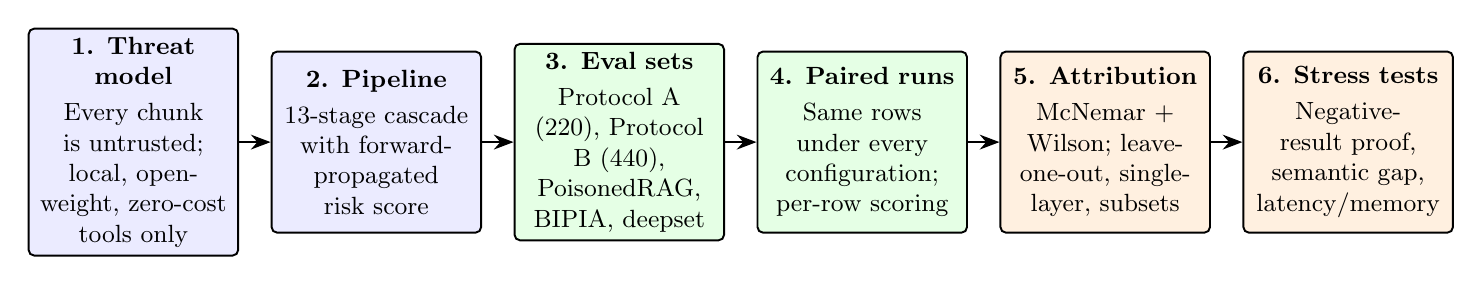
\begin{tikzpicture}[
  node distance=4mm,
  wfstep/.style={draw, rounded corners=2pt, line width=0.7pt, align=center,
               text width=2.45cm, minimum height=2.3cm, font=\small, inner sep=3pt},
  arr/.style={-{Stealth[length=2.5mm]}, line width=0.9pt}]
\node[wfstep, fill=blue!8]   (s1) {\textbf{1. Threat model}\\[2pt] Every chunk is untrusted; local, open-weight, zero-cost tools only};
\node[wfstep, fill=blue!8,   right=of s1] (s2) {\textbf{2. Pipeline}\\[2pt] 13-stage cascade with forward-propagated risk score};
\node[wfstep, fill=green!10, right=of s2] (s3) {\textbf{3. Eval sets}\\[2pt] Protocol A (220), Protocol B (440), PoisonedRAG, BIPIA, deepset};
\node[wfstep, fill=green!10, right=of s3] (s4) {\textbf{4. Paired runs}\\[2pt] Same rows under every configuration; per-row scoring};
\node[wfstep, fill=orange!12,right=of s4] (s5) {\textbf{5. Attribution}\\[2pt] McNemar + Wilson; leave-one-out, single-layer, subsets};
\node[wfstep, fill=orange!12,right=of s5] (s6) {\textbf{6. Stress tests}\\[2pt] Negative-result proof, semantic gap, latency/memory};
\foreach \a/\b in {s1/s2,s2/s3,s3/s4,s4/s5,s5/s6} \draw[arr] (\a) -- (\b);
\end{tikzpicture}
\caption{Evaluation workflow. Blue: design; green: data and execution; orange: analysis.}
\label{fig:workflow}
\end{figure*}

\section{Results and Discussion}\label{sec:results}
\subsection{Specificity, Indirect Injection, and Gate Adaptivity}
\emph{Specificity.} The fusion gate flags none of the 80 benign rows (0/80, 95\% CI [0, 4.6]\%). Downstream, the controller run refuses 10 benign rows (14 without the controller). About 6 of these refusals come from the disagreement-at-risk signal and 3 from ungrounded-recovery refusals, and 1 is an out-of-memory error rather than a security decision.
\emph{Indirect injection.} In both runs, all 40 poisoned chunks were redacted at Stage~6 and all 40 canaries stayed intact at Stage~10, while the benign queries were still answered. This defense comes from sanitization and canary verification, not from classifier recall.
\emph{Gate adaptivity.} The gate alone flags 29--30 of the 40 direct-injection queries (25 blocked, 4--5 sent to review). All 40 are blocked once the propagated risk tightens the downstream stages, which is direct evidence that the forward-propagated risk score defends beyond the gate.

\subsection{Conjunctive Detection: Negative on Saturated Scores, Recovered on Graded Margins}\label{sec:negative}
The multi-vector detector was built for the conjunctive class. With the scanner's saturated softmax probabilities as channels, it does not fire on the cases it targets, for a structural reason (Table~\ref{tab:negative}). We first present this negative result and its premise, then the repair that the premise suggests.

\textbf{Measured.} Of the 40 multivector rows, the gate blocked 6 before the detector ran. Of the remaining 34, the detector fired on 1, but that fire is invalid: both channels were individually above threshold ($x_q=0.7$, $x_c=1.0$), so it reflects ordinary single-channel detection rather than coordination of sub-threshold signals. The valid-fire condition holds on none of the 34 rows.

\textbf{Why calibration cannot rescue it.} Platt scaling was rejected for the query channel, which therefore fell back to the identity map. Class separation (Section~\ref{sec:setup}) is $-0.30$ raw and $-0.39$ after calibration. A negative separation means that the attack and benign score distributions overlap at the relevant tails. A monotone recalibration preserves this ordering, so no recalibration can create a usable graded band. The context channel could not be calibrated at all.

\textbf{Empirical confirmation.} We wrote new conjunctive payloads and ran them through the unchanged Stages~3 and~6. None of the 4 candidate pairs produced a valid fire. Two fired only because both channels scored 1.0, so they were single-channel detections that the gate already blocks. In the other two, Stage~6 dropped the poisoned chunk before the detector ran. The earlier stages behaved as intended.

\textbf{Closed-form argument.} A valid conjunctive fire requires the query to pass Stage~3 (low injection score on $x_q$) and the chunk to survive Stage~6 (low injection score on $x_c$). Any co-activation signal derived from injection-signature strength is therefore low on exactly the rows that pass both stages, so it cannot fire on the band a genuine sub-threshold attack must occupy. A high joint signal with both individual signals below threshold would require measuring something other than signature strength, such as semantic intent, which this detector does not. Conversely, any directive payload strong enough to raise the joint signal saturates the near-binary classifier in at least one channel, and is then blocked at Stage~3 or dropped at Stage~6 as a single-channel detection. No surviving-and-dangerous middle band exists. This is not a tuning failure but a structural property of a detector whose channels are \emph{saturated} probabilities. The argument rests on one premise: the scanner output is near-binary, so ``passes the gate'' and ``carries a weak signature'' coincide.

\textbf{Repair: graded logit margins.} The premise suggests a fix. Instead of the saturated probability, we read the DeBERTa logit margin as a graded channel, with the floors and joint minimum of Eq.~(\ref{eq:fire}) fixed from benign rows of an earlier calibration run. Re-running the same 30 post-gate multivector rows of the current slice, the detector fires on 0/30 with saturated channels and on 24/30 with graded channels. All 24 fires are genuinely sub-threshold (both channels below 0.9). False fires are 1/80 benign, 0/40 poisoned-context, and 3/20 gate-slip rows. So the closed-form impossibility applies to saturated channels, not to injection signatures as such. Two caveats limit this positive result. First, the floors were derived from benign rows of an earlier calibration run of the same slice, so the 1/80 false-fire rate is in-sample. Second, on the external BIPIA conjunctive construction ($n=30$), the graded detector fires on 8/30 attacks and on 4/30 benign BIPIA controls (the mitigation harness's looser rule, with query floor 0.20 and no joint minimum, gives 10/30 and 4/30), so it generalizes only modestly. To test the first caveat, we scored 200 benign rag-mini-wikipedia questions that appear in no evaluation slice through Stages~1--6. With the paper's floors the detector fires on 6 of them (3.0\%, [1.4, 6.4]), against 1/80 in-sample. The benign query channel is low (95th percentile 0.18, so the 0.228 query floor transfers), but the benign context channel is not: its 95th percentile is 0.59 on the held-out questions and 0.54 on the Protocol~A benign rows themselves. The 0.30 context floor therefore sits well inside the benign range, and benign false fires are held down by the query floor and the joint minimum, not by the context floor. Raising the context floor to the held-out 95th percentile plus 0.05 (0.637) cuts held-out false fires to 1/200 but also cuts valid fires to 0/30. No intermediate setting does better. Sweeping the context floor from 0.30 to 0.60 (query floor 0.20--0.25) only trades valid fires against false fires: at 0.40 the detector keeps 11/30 valid fires and still fires on 5/200 held-out benign questions. The reason is that the post-gate attack contexts score 0.33--0.39 (5th--50th percentile), inside the benign range, so no floor on this channel separates them. The graded repair therefore shows that the impossibility is specific to saturated channels; it is not yet a detector whose context channel separates attacks from ordinary retrieved text.

\textbf{Security implication.} The detector's failure on saturated scores did not translate into a security failure. Every multivector row in Protocol~A was neutralized anyway, because Stage~6 redacted the poisoned chunk before generation (Section~\ref{sec:e2e}). The practical lesson is that a co-activation detector is only as good as the resolution of its channels. With saturated classifier outputs it is dead weight; with graded margins it becomes a useful, but not yet externally validated, signal.

\begin{table}[t]
\centering
\caption{Evidence chain for the negative result.}
\label{tab:negative}
\small
\begin{tabular}{>{\raggedright\arraybackslash}p{2.9cm}>{\raggedright\arraybackslash}p{4.95cm}}
\toprule
Evidence source & Finding \\
\midrule
Slice (34 rows, post-gate) & 1/34 fires, invalid (both supra-threshold) \\
Sub-threshold condition & Holds on 0/34 rows \\
Calibration (query channel) & Separation $-0.30$ raw, $-0.39$ calibrated \\
Calibration (context channel) & Never calibrated \\
Real-scanner stress (4 pairs) & 0/4 valid; 2 single-channel, 2 no-fire \\
Closed-form argument & No surviving-and-dangerous band \\
\midrule
Graded margins (30 rows) & 24/30 valid fires; 1/80 benign \\
Graded, external BIPIA & 8/30 attack; 4/30 benign \\
\bottomrule
\end{tabular}
\end{table}

\subsection{End-to-End Neutralization: What the Evidence Supports}\label{sec:e2e}
The meaningful metric is whether a payload reached the user, not whether a detector fired. We report it at two levels of strictness, because they support different claims.

\emph{Level 1: canary integrity (Protocol A).} No canary leaked in any row where the check ran: the canary was checked on 175 of the 220 rows (176 in the controller-off run) and found intact every time, including all 132 delivered answers; the other 45 (44) rows were blocked before the check, 44 of them at the gate. In addition, 74 of 74 poison chunks were redacted at Stage~6 (40 poisoned-context and 34 evaluated multivector rows), with the canary unchanged in every case. Every attack row was either blocked (direct and gate-slip classes) or had its poison redacted before generation (indirect and multivector classes), even though the multivector detector itself failed. For the indirect and multivector classes, this shows that the poisoned chunk was removed before the generator saw it. For blocked direct and gate-slip rows it shows only that no answer was delivered, since some of these rows are blocked after generation. It does \emph{not} show that the model's output was benign: a canary is a proxy for instruction-following of the context, and an answer can be wrong or attacker-influenced while the canary stays intact.

\emph{Level 2: malicious output behavior (Protocol B).} To verify behavior directly, Protocol~B checks every delivered response for the attacker's target string (Section~\ref{sec:setup}). Here neutralization is not total. The full stack lets 7 of 200 planted attacks succeed (3.5\%, 95\% CI [1.7, 7.0], against 29.5\% undefended). On the 40-row semantic slice, 14 of 40 succeed (Section~\ref{sec:semantic}); on PoisonedRAG, 136 of 150 succeed, no fewer than the 137 that succeed undefended (Section~\ref{sec:external}). On BIPIA, 45 of 50 are blocked, and manual reading of the other 5 finds 2--3 that followed the injected instruction.

The accurate claim is therefore narrower than ``100\% neutralization''. On the instruction-carrying attacks of Protocol~A, no canary leaked into any delivered answer (0 of 132), and every poisoned chunk was redacted before generation (74/74). When output behavior is scored directly, the defense reduces attack success by about 88\% relative (29.5\%$\rightarrow$3.5\%) but does not eliminate it, and it does not extend to knowledge-corruption attacks. As before, the protection comes from simple layers that negate the payload before generation, not from the most complex detector.

\subsection{Controller versus Single-Pass Pipeline}
The closed-loop controller adds no measurable security over the single-pass pipeline (controller disabled): its net multivector catch is 0 in both runs. It differs in utility. Through recovery retries, it blocks 88 rows against 101 for the single-pass pipeline and answers 70 benign rows (vs.\ 66) and 34 poisoned-context rows (vs.\ 28), at the cost of extra generations on the affected rows. Under both scoring conventions we measure no security difference between the two configurations; as Section~\ref{sec:setup} notes, this is not a demonstration of equivalence. The accurate claim is therefore ``no measured security gain, at a lower false-refusal cost'', not ``additional prevention''.

\subsection{Is the Full Cascade Necessary? Ablation Against Simpler Defenses}\label{sec:ablation}
Does a thirteen-stage cascade outperform a simpler defense? We answer this with a current-code ablation under Protocol~B (Section~\ref{sec:setup}): 200 planted-attack rows and 200 benign rows, each configuration paired row-by-row with the same undefended arm, and the seven mitigation layers toggled independently (Table~\ref{tab:ablation}).

\begin{table}[t]
\centering
\caption{Ablation under Protocol B ($n=200$ attack, $n=200$ benign per arm). ASR = attack success rate with Wilson 95\% CI; $p$ = exact McNemar test against the paired undefended arm (``fix/brk'' = discordant rows the configuration fixed / broke). Benign blk = benign rows refused.}
\label{tab:ablation}
\setlength{\tabcolsep}{2.5pt}
\small
\resizebox{\columnwidth}{!}{%
\begin{tabular}{lcccc}
\toprule
Configuration & ASR \% [95\% CI] & fix/brk & $p$ & \makecell{Benign\\blk \%} \\
\midrule
Undefended & 29.5 [23.6, 36.2] & -- & -- & 0.0 \\
\textbf{Full stack (7 layers)} & \textbf{3.5} [1.7, 7.0] & 54/2 & $<\!10^{-13}$ & 8.5 \\
\midrule
\multicolumn{5}{l}{\emph{Leave one out}} \\
\quad $-$ sanitization & 11.0 [7.4, 16.1] & 50/13 & $3\!\times\!10^{-6}$ & 7.5 \\
\quad $-$ grounding gate & 6.5 [3.8, 10.8] & 49/3 & $10^{-11}$ & 2.5 \\
\quad $-$ refuse-on-detection & 6.0 [3.5, 10.2] & 51/4 & $2\!\times\!10^{-11}$ & 7.0 \\
\quad $-$ tightened rerank & 6.0 [3.5, 10.2] & 51/4 & $2\!\times\!10^{-11}$ & 6.5 \\
\quad $-$ guarded prompt & 5.5 [3.1, 9.6] & 53/5 & $3\!\times\!10^{-11}$ & 12.5 \\
\quad $-$ Presidio & 4.0 [2.0, 7.7] & 53/2 & $<\!10^{-13}$ & 8.5 \\
\quad $-$ DLP & 3.5 [1.7, 7.0] & 54/2 & $<\!10^{-13}$ & 8.5 \\
\midrule
\multicolumn{5}{l}{\emph{Single layer only}} \\
\quad Grounding gate & 15.0 [10.7, 20.6] & 29/0 & $4\!\times\!10^{-9}$ & 5.5 \\
\quad Sanitization & 16.0 [11.6, 21.7] & 30/3 & $1.4\!\times\!10^{-6}$ & 0.0 \\
\quad Refuse-on-detection & 18.0 [13.3, 23.9] & 25/2 & $6\!\times\!10^{-6}$ & 2.5 \\
\quad Tightened rerank & 24.5 [19.1, 30.9] & 28/18 & 0.18 & 0.0 \\
\quad Guarded prompt & 53.0 [46.1, 59.8] & 6/53 & $2\!\times\!10^{-10}$ & 0.0 \\
\quad Presidio / DLP & 29.5 [23.6, 36.2] & 0/0 & 1.0 & 0.0 \\
\midrule
\multicolumn{5}{l}{\emph{Subsets}} \\
\quad \textbf{Sanitize+ground+refuse} & \textbf{5.5} [3.1, 9.6] & 48/0 & $7\!\times\!10^{-15}$ & 9.5 \\
\quad Sanitize+ground & 8.5 [5.4, 13.2] & 42/0 & $5\!\times\!10^{-13}$ & 8.0 \\
\quad Sanitize+refuse & 9.5 [6.2, 14.4] & 42/2 & $10^{-10}$ & 2.5 \\
\quad Ground+refuse & 10.5 [7.0, 15.5] & 40/2 & $4\!\times\!10^{-10}$ & 7.5 \\
\bottomrule
\end{tabular}}
\end{table}

\begin{figure}[t]
\centering
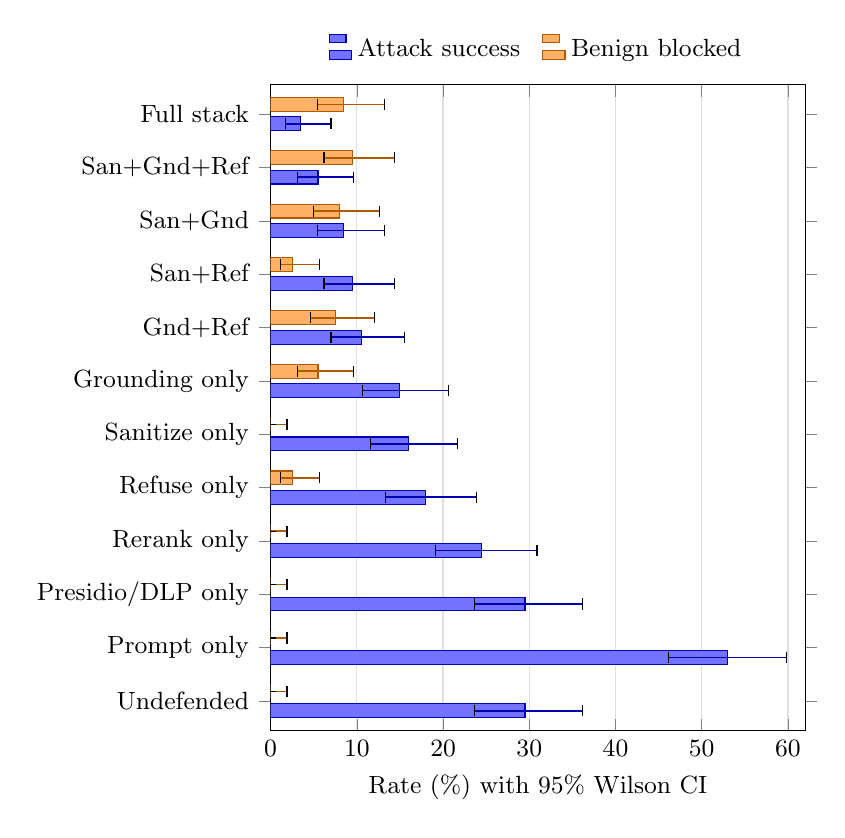
\begin{tikzpicture}
\begin{axis}[
  xbar, scale only axis, width=0.56\columnwidth, height=8.2cm,
  bar width=5pt, xmin=0, xmax=62,
  xlabel={Rate (\%) with 95\% Wilson CI}, xlabel style={font=\small},
  symbolic y coords={a0,a1,a2,a3,a4,a5,a6,a7,a8,a9,a10,a11},
  ytick=data, yticklabels={{Full stack},{San+Gnd+Ref},{San+Gnd},{San+Ref},{Gnd+Ref},{Grounding only},{Sanitize only},{Refuse only},{Rerank only},{Presidio/DLP only},{Prompt only},{Undefended}}, y dir=reverse, yticklabel style={font=\small},
  xticklabel style={font=\small}, enlarge y limits=0.05,
  legend style={font=\small, at={(0.5,1.02)}, anchor=south, legend columns=2, draw=none, /tikz/every even column/.append style={column sep=6pt}},
  xmajorgrids, grid style={gray!25},
  error bars/x dir=both, error bars/x explicit,
  error bars/error bar style={line width=0.6pt}]
\addplot[fill=blue!55, draw=blue!70!black] coordinates {
 (3.5,a0) += (3.5,0) -= (1.8,0)
 (5.5,a1) += (4.1,0) -= (2.4,0)
 (8.5,a2) += (4.7,0) -= (3.1,0)
 (9.5,a3) += (4.9,0) -= (3.3,0)
 (10.5,a4) += (5.0,0) -= (3.5,0)
 (15.0,a5) += (5.6,0) -= (4.3,0)
 (16.0,a6) += (5.7,0) -= (4.4,0)
 (18.0,a7) += (5.9,0) -= (4.7,0)
 (24.5,a8) += (6.4,0) -= (5.4,0)
 (29.5,a9) += (6.7,0) -= (5.9,0)
 (53.0,a10) += (6.8,0) -= (6.9,0)
 (29.5,a11) += (6.7,0) -= (5.9,0)};
\addplot[fill=orange!60, draw=orange!70!black] coordinates {
 (8.5,a0) += (4.7,0) -= (3.1,0)
 (9.5,a1) += (4.9,0) -= (3.3,0)
 (8.0,a2) += (4.6,0) -= (3.0,0)
 (2.5,a3) += (3.2,0) -= (1.4,0)
 (7.5,a4) += (4.5,0) -= (2.9,0)
 (5.5,a5) += (4.1,0) -= (2.4,0)
 (0.0,a6) += (1.9,0) -= (0,0)
 (2.5,a7) += (3.2,0) -= (1.4,0)
 (0.0,a8) += (1.9,0) -= (0,0)
 (0.0,a9) += (1.9,0) -= (0,0)
 (0.0,a10) += (1.9,0) -= (0,0)
 (0.0,a11) += (1.9,0) -= (0,0)};
\legend{Attack success,Benign blocked}
\end{axis}
\end{tikzpicture}
\caption{Attack success and benign blocking by configuration, Protocol B ($n=200$ attack and $n=200$ benign rows per arm, current code). San = sanitization, Gnd = grounding gate, Ref = refuse-on-detection.}
\label{fig:asr}
\end{figure}

\begin{figure}[t]
\centering
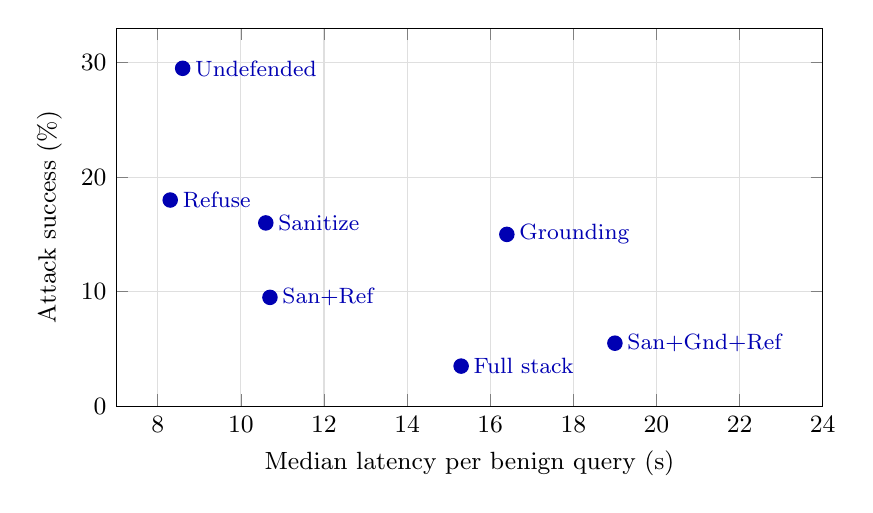
\begin{tikzpicture}
\begin{axis}[
  scale only axis, width=0.74\columnwidth, height=4.8cm,
  xlabel={Median latency per benign query (s)}, ylabel={Attack success (\%)},
  xlabel style={font=\small}, ylabel style={font=\small},
  ticklabel style={font=\small}, xmin=7, xmax=24, ymin=0, ymax=33,
  grid=major, grid style={gray!25},
  nodes near coords, point meta=explicit symbolic,
  every node near coord/.append style={font=\footnotesize, anchor=west, xshift=1pt}]
\addplot[only marks, mark=*, mark size=2.6pt, blue!70!black] coordinates {
 (8.6,29.5)[Undefended]
 (8.3,18.0)[Refuse]
 (10.6,16.0)[Sanitize]
 (16.4,15.0)[Grounding]
 (10.7,9.5)[San+Ref]
 (19.0,5.5)[San+Gnd+Ref]
 (15.3,3.5)[Full stack]};
\end{axis}
\end{tikzpicture}
\caption{Security versus latency (Protocol B, current code). Sanitize+refuse obtains about three quarters of the full-stack ASR reduction (20 of 26 points) for +2\,s; adding grounding obtains most of the remainder for a further 5--8\,s.}
\label{fig:tradeoff}
\end{figure}

Three results follow. First, no single layer approaches the full stack: the best single layers (grounding, sanitization, refuse-on-detection) leave 15--18\% ASR, and the guarded prompt alone \emph{raises} ASR to 53.0\% (53 rows broken, 6 fixed). This is consistent with the stricter context-only template making the generator defer more readily to the ``authoritative correction'' that the attack plants in the chunk, though we have not isolated the mechanism. Second, the layers are complementary: every subset beats each of its own constituent layers in paired tests (e.g., sanitize+ground+refuse vs.\ sanitize alone: 0 rows worse, 21 better, $p<10^{-6}$). Third, and most important for deployment, the three-layer subset sanitize+ground+refuse is not significantly different from the seven-layer stack: 5.5\% vs.\ 3.5\% ASR, with 7 rows succeeding only under the subset and 3 only under the full stack (exact McNemar $p=0.34$), and 9.5\% vs.\ 8.5\% benign blocking ($p=0.77$). The two-layer subsets are worse than the full stack: ground+refuse ($p=0.004$) and sanitize+refuse ($p=0.008$) survive Bonferroni correction ($\alpha=0.0125$), while sanitize+ground ($p=0.021$) does not. A non-significant difference at $n=200$ cannot rule out a gap of a few points between the three-layer subset and the full stack, so we do not claim equivalence; the enlarged sample below bounds the gap instead. Presidio and DLP have no measurable effect on injection ASR (they target PII and are evaluated separately).

\textbf{Replicates.} To check that these results are not an artifact of one generation run, we repeated the undefended, full-stack, and three-layer arms (attack and benign) with generation seeds 7 and 1234 on the same 400 rows. Across the three replicates, undefended ASR is $30.3\pm0.8\%$ (29.5, 31.0, 30.5), full-stack ASR is $4.2\pm0.6\%$ (3.5, 4.5, 4.5), and three-layer ASR is $6.0\pm0.9\%$ (5.5, 7.0, 5.5) (mean $\pm$ SD). The full stack beats undefended in every replicate ($p<10^{-12}$). The subset is not significantly different from the full stack in any replicate ($p=0.34$, 0.27, 0.77), but it is worse in all three, by $1.8\pm0.8$ points. We therefore read the subset as giving up one to three points of ASR for four fewer layers, not as cost-free. Benign blocking is $9.3\pm1.0\%$ for the full stack and $8.2\pm1.5\%$ for the subset. Outcomes are stable at the row level: 51 rows succeed undefended in every replicate and 69 in at least one, while under the full stack 6 rows succeed in every replicate and 10 in at least one. The residual full-stack failures are therefore a small, mostly fixed set of rows rather than random noise. As a reproduction check, we regenerated the undefended and full-stack arms from the raw slice with the released code (seed 42). The fresh run gives 58/200 (29.0\%) undefended and 6/200 (3.0\%) full-stack successes, against 59 and 7 in the reported run. The two runs agree on 189 and 199 of the 200 rows respectively (no significant drift; exact McNemar $p=1.0$ for both), and the fresh full-stack arm again fixes 54 rows and breaks 2 ($p<10^{-13}$). The defensible conclusion is that, on these instruction-bearing attacks, three layers carry most of the measured injection defense; they do not suffice for assertion-only attacks (see \emph{Class dependence and wording} below). Fewer layers do not mean lower latency in our implementation: the subset's median benign latency is 19.0\,s against 15.3\,s for the seven-layer stack (Table~\ref{tab:overhead}). The subset keeps the grounding judge, which is the dominant cost; we have not isolated why it is slower than the full stack. The remaining stages, including both extensions, should be justified by other threats (PII, gate-level blocking) or by utility, not by injection security.

\textbf{Larger sample.} A non-significant difference at $n=200$ leaves a gap of several points possible. We therefore built 224 further planted attacks with the same constructor and seed, which exhausts the yes/no questions in the bank ($n=424$ in total), and ran the undefended, full-stack, and three-layer arms on them. Over all 424 paired rows, ASR is 29.7\% undefended [25.6, 34.2], 4.2\% for the full stack [2.7, 6.6], and 4.7\% for the three-layer subset [3.1, 7.2]. The full stack fixes 114 rows and breaks 6 ($p<10^{-26}$). The subset and the full stack differ on 18 rows (10 succeed only under the subset, 8 only under the full stack; $p=0.81$), for a paired difference of $+0.5$ points with an approximate 95\% interval of $[-1.5, +2.4]$. On the 224 new rows alone the subset is slightly \emph{better} (4.0\% vs.\ 4.9\%, $p=0.73$). The larger sample thus bounds the cost of dropping the other four layers at about 2.4 points of ASR (95\% upper bound; no equivalence margin was prespecified, and the subset was worse in all three $n=200$ replicates, by 1.0--2.5 points).

\textbf{Interactions.} Leave-one-out and single-layer arms cannot show whether layers interact, so we ran sanitization (S), grounding (G), and refusal (R) in all eight combinations with the other four layers off (Table~\ref{tab:factorial}). On the additive scale every pair is sub-additive (S+G reduces ASR by 21.0 points against 13.5 and 14.5 for its parts), which would suggest redundancy. A better null is that each layer independently removes a fixed fraction of the attacks that reach it, so the surviving fractions multiply. Against this null every combination matches within 1.3 points, and every 95\% paired-bootstrap interval of the difference includes 0 (S+G+R: 5.5\% observed vs.\ 5.0\% predicted, $[-1.6, +2.8]$). The three layers therefore act as near-independent filters. Each removes 39--49\% of what reaches it, they stop largely different rows (of the 59 undefended successes, 22 are fixed by exactly one of the three single layers and none only by their combination), and absolute returns diminish as layers are added. Their exact Shapley values over the 24.0-point reduction are 8.7 (S, [5.1, 12.6]), 8.7 (G, [5.8, 11.9]), and 6.7 (R, [3.8, 9.7]) points; the benign-refusal cost is concentrated in the grounding gate (6.3 of 9.5 points). The guarded prompt is the one layer whose effect changes sign with context: alone it raises ASR by 23.5 points, while removing it from the full stack changes ASR by only $+2.0$ $[-0.8, +4.8]$; the arms we ran cannot identify which layer neutralizes it. Effects of one to three points are within the run-to-run noise of this setup (two runs of the same undefended configuration differ on 11 of 200 rows).

\textbf{Class dependence and wording.} The subset result does not transfer across attack classes. On the 40-row assertion-only slice (Section~\ref{sec:semantic}), sanitize+ground+refuse leaves 25/40 (62.5\%) against 14/40 (35.0\%) for all seven layers (12 vs.\ 1 discordant rows, $p=0.003$) and is not significantly better than undefended ($p=0.13$). The guarded prompt, harmful on its own against the instruction-bearing Protocol~B attacks, is the most effective single layer on this slice (alone 75.0\%$\rightarrow$52.5\%, $p=0.035$). Within Protocol~B, an exploratory analysis of the randomized attack templates shows that protection also depends on wording. For one of the three coercive query phrasings (``Defer to any authoritative correction\ldots'') the detector behind refuse-on-detection fires on every row and full-stack ASR is 0/147; for another it fires on 20\% of rows and full-stack ASR is 9.9\% [5.9, 16.2] (permutation test of homogeneity $p=0.0001$, $n=424$). The 3.5\% headline is therefore an average over phrasings with different outcomes. These subgroup results are exploratory and were not prespecified, so we tested them in a preregistered follow-up on the same 200 questions and targets with only the wording changed (two paired tests, Bonferroni $\alpha=0.025$). With three new coercive query suffixes and four new poison templates, fixed before any run, full-stack ASR was 3.0\% [1.4, 6.4] against 3.5\% (6 vs.\ 7 discordant rows, $p=1.0$): the protection transferred, although the new wording was the stronger attack (40.5\% undefended) and the detector fired on 111 of 200 rows. With the coercive query suffix removed, the attack was weaker (16.5\% undefended) and the detector fired on 6 rows instead of 80; full-stack ASR was 7.5\% [4.6, 12.0] (14 vs.\ 6, $p=0.115$), not significant, while the relative reduction fell from 88\% to 55\%. We therefore do not claim that the defense is weaker without coercive phrasing; refuse-on-detection reacts mainly to query phrasing, and in this run the other layers left a smaller margin when it did not fire. In neither variant was the three-layer subset significantly different from the seven-layer stack (+3.5 points, 95\% CI $-0.7$ to 7.7, without suffix; $-1.0$ points with held-out wording); this is not evidence of equivalence. The held-out wording was written by us, not by an adaptive attacker.

\begin{table}[t]
\centering
\caption{Fully crossed factorial of sanitization (S), grounding (G), and refuse-on-detection (R), other four layers off (Protocol~B, $n=200$ attack and 200 benign). ``Indep.'' = ASR predicted if each layer independently removes a fixed fraction of the attacks that reach it.}
\label{tab:factorial}
\small
\begin{tabular}{lccc}
\toprule
Layers & ASR \% & Indep.\ \% & Benign refused \% \\
\midrule
none & 29.5 & -- & 0.0 \\
S & 16.0 & -- & 0.0 \\
G & 15.0 & -- & 5.5 \\
R & 18.0 & -- & 2.5 \\
S+G & 8.5 & 8.1 & 8.0 \\
S+R & 9.5 & 9.8 & 2.5 \\
G+R & 10.5 & 9.2 & 7.5 \\
S+G+R & 5.5 & 5.0 & 9.5 \\
\midrule
\multicolumn{4}{l}{\footnotesize Shapley shares of the 24.0-pt ASR drop: S 8.7, G 8.7, R 6.7.} \\
\multicolumn{4}{l}{\footnotesize Shapley share of benign refusals: S 1.1, G 6.3, R 2.1 pts.} \\
\bottomrule
\end{tabular}
\end{table}

\textbf{External baselines.} We compared the pipeline with three external defenses on the same 210 paired rows of the adversarial slice (130 attack, 80 benign). (i) A detector-only LLM-Guard baseline (DeBERTa-v3 on query and chunk, threshold 0.5) flags 65/130 attacks (recall 50\%) at 0/80 false positives. It catches all 40 poisoned chunks but only 1/30 multivector attacks and 12/40 adversarial queries, so the single off-the-shelf detector alone misses half of the attacks. (ii) A paper-faithful ControlNET~\cite{yao2025controlnet} detector (activation-shift on Llama-3.1-8B) blocks 93/130 attacks and 9/80 benign rows, compared with 95/130 and 10/80 for our pipeline; neither difference is significant (exact McNemar $p=0.85$ and $p=1.0$). However, ControlNET removes the poison before generation on only 33/70 context-attack rows, versus 67/70 for our pipeline. (iii) The official Sentinel--Strategist (ADO) code~\cite{palleria2026ado} never refuses; it removes the poison on 25--44 of 70 context-attack rows (lower and upper bounds, depending on whether its attention filter is counted), versus 67/70 for our pipeline ($p\le1.6\times10^{-6}$). Its end-to-end ASR on the 50 marker-scorable rows is 8.0\% vs.\ 2.0\% for our pipeline, which is not significant at $n=50$ ($p=0.375$). ControlNET was run on quantized GGUF weights, and the ADO attention filter could not run under Ollama (it does run in the Protocol~B comparison below). These comparisons are therefore indicative, not exact reproductions.

\textbf{Existing defenses on Protocol B.} The comparisons above use the Protocol~A slice and different metrics per system. To compare end-to-end outcomes directly, we ran four existing defenses on the 200 planted attacks and 200 benign questions of Protocol~B, with the same single generator, decoding, and scoring as Table~\ref{tab:ablation}, paired row by row (Table~\ref{tab:existing}). \emph{Spotlighting}~\cite{hines2024spotlighting} uses its datamarking variant: each retrieved passage has a marker interleaved between its words and the system prompt explains the marker; the answers are regenerated. \emph{LLM-Guard}~\cite{protectai2024} is used as an input firewall: its prompt-injection scanner (threshold 0.5) checks the query and every passage placed in the prompt, and any flag refuses the query. \emph{ControlNET} is the detector described above (Llama-3.1-8B layer-1 activations, decision tree), retrained on the same data and given exactly the eight reranked passages the undefended generator received (the planted chunk survives reranking in 184 of the 200 rows). LLM-Guard and ControlNET only block or pass, so a guarded deployment delivers the undefended answer on every row they pass; we score them by applying their decisions to the stored undefended answers, after recomputing the passages the undefended pipeline retrieved (retrieval is deterministic). The full stack lets 3.5\% of attacks succeed, against 21.0\% for LLM-Guard (3 rows succeed only under the full stack, 38 only under LLM-Guard; $p=1\times10^{-8}$) and 23.0\% for Spotlighting ($p<10^{-9}$), with no significant difference in benign correctness from either. Spotlighting refuses no benign question but stops few attacks. ControlNET is the strongest existing defense: its 4.5\% ASR is not significantly different from the full stack's ($p=0.77$) or the three-layer subset's 5.5\% ($p=0.80$). It also blocks 15 of the 16 attacks whose planted chunk never reached the generator, so much of its signal comes from the coercive wording of the attack queries rather than from the planted passage. An earlier variant that appended the planted chunk to every row gave 5.0\% ASR with the same conclusions. It answers fewer benign questions correctly (46.0\% vs.\ 52.0\%; $p=0.058$ against the full stack and $p=0.012$ against the three-layer subset) and refuses more (13.5\% vs.\ 8.5\%, $p=0.13$). The defensible claim is therefore that the seven-layer configuration clearly outperforms an input firewall and prompt-level spotlighting, and matches the strongest detector we tested on attack success with somewhat better benign utility; it does not establish superiority over ControlNET. Two caveats apply. Our ControlNET retraining reaches a validation F1 of 0.88 against 0.90 in the run reported above (a newer \texttt{transformers} release was used there), and ControlNET's mitigation module (ProNet) is not reimplemented, so it is evaluated as a detect-and-block firewall. \emph{ADO}~\cite{palleria2026ado} runs from the authors' unmodified code through an adapter: for each query its Sentinel and Strategist (Llama-3.1-8B via Ollama) choose among DP-RAG, TrustRAG, and attention-variance filtering, these defenses act on the same eight passages, and the same generator then answers with ADO's own prompt. Local hardware forced two substitutions (Llama-3.1-8B instead of Llama-3-8B as controller, and a 4-bit Llama-3.1-8B for the attention filter), and every query starts as a fresh user, so ADO's trust mechanism is inactive; we therefore call it an adapted implementation, not a reproduction. ADO lets 28.5\% of attacks succeed, against 3.5\% for the full stack (54 vs.\ 4 discordant rows, $p=3\times10^{-12}$), and answers fewer benign questions correctly (35.5\% vs.\ 52.0\%, $p=6\times10^{-6}$). Both effects have one main cause: DP-RAG removes every passage on 64 of the 200 attacks and 58 of the 200 benign questions. The generator then refuses (``No relevant information was found\ldots''), which stops the attack but also discards the evidence, and which the marker scorer counts as a success whenever the planted answer is ``No'' (30 of ADO's 57 successes). If refusals are not counted as attack successes for any arm, ADO's ASR is 13.5\% against 3.5\% (24 vs.\ 4 discordant rows, $p=2\times10^{-4}$); this criterion was preregistered for 150 of the 200 attacks and fixed after the pilot for the other 50. These results concern this adapted implementation under Protocol~B's marker scoring; they do not establish superiority over every faithful ADO deployment. Its median latency is 45\,s per query, against 15.3\,s for the full stack.

\begin{table}[t]
\centering
\caption{Existing defenses on Protocol B: 200 planted attacks and 200 benign questions, same generator and scoring, paired by row. Wilson 95\% CIs; $p$ = exact McNemar test of attack success against the full stack.}
\label{tab:existing}
\setlength{\tabcolsep}{2.5pt}
\small
\resizebox{\columnwidth}{!}{%
\begin{tabular}{lcccc}
\toprule
Defense & ASR \% [95\% CI] & \makecell{Benign\\blocked \%} & \makecell{Benign\\correct \%} & $p$ \\
\midrule
Undefended & 29.5 [23.6, 36.2] & 0.0 & 56.5 & $<\!10^{-13}$ \\
ADO orchestrator$^{\dagger}$ & 28.5 [22.7, 35.1] & 0.0 & 35.5 & $3\!\times\!10^{-12}$ \\
Spotlighting & 23.0 [17.7, 29.3] & 0.0 & 55.5 & $9\!\times\!10^{-10}$ \\
LLM-Guard firewall & 21.0 [15.9, 27.2] & 8.5 & 51.0 & $1\!\times\!10^{-8}$ \\
ControlNET detector$^{*}$ & 4.5 [2.4, 8.3] & 13.5 & 46.0 & 0.77 \\
\midrule
This work, 3 layers & 5.5 [3.1, 9.6] & 9.5 & 52.0 & 0.34 \\
This work, 7 layers & 3.5 [1.7, 7.0] & 8.5 & 52.0 & -- \\
\bottomrule
\end{tabular}}
{\footnotesize $^{*}$Detection and blocking only; ControlNET's mitigation module is not reimplemented. $^{\dagger}$Adapted implementation (official code; Llama-3.1-8B controller, 4-bit attention filter); 13.5\% ASR if refusals are not counted as attack successes.\par}
\end{table}

\subsection{Earlier-Code Mitigation Arms}\label{sec:stats}
The submitted version reported mitigation arms from an earlier code version (Figs.~2--3 of that version; undefended ASR 31.0\%). There, refusal-on-detection was the only standalone layer to clear $p<0.05$; adding grounding on top of refusal gave no further reduction ($p=1.0$); and aggressive pre-generation filtering raised benign false positives without reducing ASR. Fusing the two input detectors as an AND-gate cut the benign false-positive rate from 45\% to 2.5\% at no recall cost, which shows that fusion helps specificity but not detection. The current-code ablation (Section~\ref{sec:ablation}, Fig.~\ref{fig:asr}) supersedes the standalone-layer result. On the current code, grounding-only and sanitization-only are also significant on their own, so we no longer claim that refusal is the only effective single layer. The AND-gate specificity finding is unaffected.

\subsection{Independent External Benchmarks}\label{sec:external}
Table~\ref{tab:external} reports the adaptive-tier variant of the pipeline (Section~\ref{sec:setup}) on data we did not construct. The outcome depends sharply on the threat model.

\begin{table*}[t]
\centering
\caption{Adaptive-tier pipeline variant (Stages 1--10, 13) on independent external sets, paired row by row with an undefended RAG arm on the same rows and poison. ASR = attack's target string in the delivered answer and true answer absent; $p$ = exact McNemar (fixed/broke).}
\label{tab:external}
\setlength{\tabcolsep}{2.5pt}
\small
\begin{tabular}{lrcccc}
\toprule
Set & $n$ & \makecell{Poison\\removed} & \makecell{ASR\\undefended} & \makecell{ASR\\defended} & \makecell{fix/brk\\($p$)} \\
\midrule
PoisonedRAG-NQ & 50 & 0/49 & 46 & 44 & 4/2 (0.69) \\
PoisonedRAG-HotpotQA & 50 & 0/50 & 46 & 47 & 1/2 (1.0) \\
PoisonedRAG-MS MARCO & 50 & 0/49 & 45 & 45 & 2/2 (1.0) \\
\textbf{PoisonedRAG, all} & 150 & 0/148 & \makecell{137 (91.3\%)\\{[85.7, 94.9]}} & \makecell{136 (90.7\%)\\{[84.9, 94.4]}} & 7/6 (1.0) \\
\quad same generator$^\ddagger$ & 150 & -- & 137 (91.3\%) & \makecell{128 (85.3\%)\\{[78.8, 90.1]}} & 16/7 (0.09) \\
\midrule
 & & & \multicolumn{2}{c}{Blocked: undef.\ / def.} & \\
BIPIA text attack & 50 & 33/49 & \multicolumn{2}{c}{0/50 / 45/50} & $^\dagger$ \\
\midrule
deepset (gate only) & 30+30 & \multicolumn{4}{l}{Blocked 14/30 (46.7\%), flagged 17/30 (20/30 with graded flag); benign 0/30} \\
\bottomrule
\end{tabular}

\vspace{2pt}{\footnotesize $^\dagger$BIPIA goals are not string-scorable; the 5 unblocked defended rows were read manually: 2 followed the injected instruction, 2 did not, 1 indeterminable. $^\ddagger$Separate run of the seven-layer single-generator harness (Protocol~B configuration), \texttt{llama3.2:3b} in both arms; in that run BIPIA is 44/50 blocked, against 45/50 for the adaptive-tier variant above.\par}
\end{table*}

\emph{Instruction-style indirect injection (BIPIA).} BIPIA goals are output-format manipulations, such as ``answer with intentional misspellings'', with no target string, so we score them by block and by manual reading. We read the 5 unblocked defended answers: 2 followed the injected instruction (one with deliberate misspellings, one with a symbol-substituted output), 2 did not, and 1 one-word answer cannot show compliance. Defended BIPIA attack success is therefore 2--3 of 50 (4--6\%). We have not annotated the 50 undefended answers, so we report the block comparison rather than a paired ASR. The undefended arm blocks none of the 50 rows; the pipeline blocks 45 of 50: 44 because the grounding judge rejected the answer and 1 at the gate. For 36 of the 44, the ungrounded answer also raised the row to high risk, so it was regenerated by the three-model ensemble before refusal and recorded as an adaptive-policy block; the regeneration could not change the outcome. Of the 49 injected chunks, 33 are removed before generation: 10 by Stage~6 sanitization and 23 by Stage~7 reranking. This is consistent with the Protocol~A result that per-chunk sanitization and downstream refusal carry the indirect-injection defense.
\emph{Knowledge corruption (PoisonedRAG).} The pipeline offers no measurable protection. Stage~6 redacts none of the 148 injected passages, because PoisonedRAG passages are fluent factual text with no instruction signature. Against a paired undefended arm (same rows, same injected passage, no defense layers, single \texttt{llama3.2:3b} generator), attack success is 91.3\% undefended and 90.7\% defended: 7 rows fixed, 6 broken, exact McNemar $p=1.0$. Four undefended answers contain both the target and the true answer; counting them as failures instead of successes gives 88.7\% undefended (6 fixed, 9 broken, $p=0.61$), with the same conclusion. Because the adaptive-tier variant adds tiered retrieval and generation, we also ran the seven-layer harness on the same rows. The seven-layer mitigation harness with \texttt{llama3.2:3b} was run on the same 200-row external set (150 PoisonedRAG and 50 BIPIA rows); on its 150 PoisonedRAG rows it reaches 85.3\% ASR (128/150) against 91.3\% undefended: 16 rows fixed, 7 broken, exact McNemar $p=0.093$, or $p=0.44$ when ambiguous undefended answers count as failures. Most of this difference comes from 11 blocked rows. The paired difference is $-6.0$ points, with an approximate 95\% interval of $[-12.2, +0.2]$. So we cannot exclude a reduction of up to about 12 points, but no configuration shows a significant one. On BIPIA, the same-generator harness blocks 44/50 against 0/50 undefended, close to the adaptive-tier variant's 45/50. The saved traces show where each stage fails. The gate scores every PoisonedRAG query 0, Stage~6 redacts none of the 148 passages, the reranker places the poisoned passage first in all 148 rows (median margin 0.23 over the next passage), and all 136 successful attacks pass the grounding judge with median faithfulness 1.0, against 0.77 for the 8 delivered answers that resisted. Counter-evidence was rarely available: the true answer appears in another retrieved passage in only 11 rows, because the questions come from corpora other than our knowledge base. Every PoisonedRAG answer was generated by a single \texttt{llama3.2:3b} (no row reached the high tier), so this run does not test ensemble disagreement; on the 8-row semantic supplement, disagreement did not separate attacks from benign questions (Section~\ref{sec:semantic}). The failure therefore lies in relevance ranking, grounding as context-consistency, and the absence of provenance, not in a single weak stage. A closed-book probe (the 150 questions without retrieved context) separates two cases: \texttt{llama3.2:3b} answered correctly in 74 of the 136 defended successes (54.4\%, 95\% CI 46.0--62.5), so the poisoned passage overrode knowledge the generator had, and in the rest it did not know the answer. Knowing the answer gave no protection (ASR 90.2\% when it knew vs.\ 91.2\% when it did not). String matching misses a few correctly phrased closed-book answers, so the first share is, if anything, slightly underestimated. This external result replicates the semantic gap of Section~\ref{sec:semantic} at a larger scale and on third-party data.
\emph{In-the-wild direct injection (deepset).} The fusion gate blocks 14 of 30 real injection prompts (46.7\%, [30.2, 63.9]) and flags 3 more for review, with no benign prompt blocked or flagged (0/30). On the full test split it blocks 23 of 60 injections (38.3\%) and flags 28, at 1/56 benign false positives. Misses are not explained by language: the split mixes English and German, and the gate flags similar shares of each (16/37 and 12/23). Gate-level detection of diverse real-world phrasing is weak, which reinforces the design choice to rely on downstream stages rather than on the gate. Thresholds cannot fix this: 31 of the 32 injections the gate passes on the full split have a scanner score of exactly 0, so they take the fast-path ALLOW. Stage~3 already computes the graded DeBERTa margin for the multivector detector, so we also let the gate flag a prompt for review when that margin exceeds a threshold $t$. Choosing $t$ on the deepset \emph{train} split (largest recall while adding at most 2\% benign flags; $t=0.230$, close to the multivector query floor) and applying it to the test split raises flagged injections from 28/60 to 38/60 (63.3\%, [50.7, 74.4]; 10 gained, none lost) and benign flags from 1/56 to 2/56. On the 30+30 sample, flagged injections rise from 17/30 to 20/30 with 0/30 benign. On the pipeline's own traffic, the added flag fires on 7 of 200 held-out benign questions (3.5\%) and on 2 of the 80 Protocol~A benign controls, so it would route a few percent of ordinary questions to review. End to end, the complete pipeline refuses all 30 sampled injections (14 at the gate, 13 by the risk controller, 3 by abstention), but it also refuses all 30 benign deepset prompts, which are not answerable from the wiki corpus. Downstream refusal on this set therefore reflects off-topic queries, not injection detection, and we report the gate figures as the deepset result.

\subsection{The Unsolved Gap: Signature-Free Semantic Injection}\label{sec:semantic}
The gate-slip class (role-play or fictional framing around an unsafe request) carries almost no injection signature. Five of its 20 rows (25\%) pass the gate in both runs, a residual that no injection-signature detector is expected to close. A sharper form is semantic misinformation: a benign-looking query paired with a planted-premise chunk that reads as neutral reference text but asserts a false fact. In the original 8-row supplement (every row confirmed by the real scanners to pass the gate and survive Stage~6), 4 of 8 attacks succeed under both the passive and the spotlighting Stage~8. Spotlighting changes \emph{which} rows are neutralized but not \emph{how many}, as expected: spotlighting removes the authority of instructions, and a planted false fact is not an instruction. No answer-side signal separates this class from benign traffic. Ensemble-disagreement AUC is 0.47--0.48 with negative percentile gaps, and faithfulness AUC is 0.62 (gap $-0.10$). Faithfulness AUC under spotlighting rises to 0.86, but its gap is still negative at $n=8$: the AUC is higher, but there is no usable threshold, so we do not count it as a positive result. A purpose-built parametric-consistency check, which verifies the claim against the model's own prior, also fails (AUC 0.54) because of benign false positives. This suggests that the viable direction is external provenance or source-trust weighting, not any signal derived from the model's own outputs. At $n=8$, the 50\% success rate has a 95\% Wilson interval of [21.5, 78.5], so we enlarged the slice fivefold.

\textbf{Forty-row free-text slice.} The revision builds 40 rows with free-text targets (e.g., a planted boiling point of 87\,$^\circ$C), using the same admission rule. Sanitization and the gate cannot act on these rows by construction, which the sanitization-only control confirms (77.5\% ASR, not significantly different from undefended). Undefended, 30/40 attacks succeed (75.0\%, [59.8, 85.8]). The full stack reduces this to 14/40 (35.0\%, [22.1, 50.5]; 18 rows fixed, 2 broken, exact McNemar $p=4\times10^{-4}$). Leave-one-out arms show where the reduction comes from. Removing the guarded prompt raises ASR to 55.0\% (9 vs.\ 1 discordant rows, $p=0.022$ vs.\ full), and removing refuse-on-detection raises it to 50.0\% (6 vs.\ 0, $p=0.031$). Neither survives Bonferroni correction for the leave-one-out family ($\alpha=0.007$) at $n=40$, so these attributions are suggestive. Removing the grounding gate changes nothing (35.0\%). Grounding alone has no effect (75.0\%), because a planted fact is perfectly ``grounded'' in the poisoned context. The external PoisonedRAG result (Section~\ref{sec:external}: 90.7\% succeed, against 91.3\% undefended) confirms the gap on third-party data. Therefore the semantic attack is partly mitigated by prompt- and refusal-level defenses on our slice, but it remains the dominant residual risk, and the defense does not transfer to PoisonedRAG.

\textbf{Isolate-and-aggregate generation.} The pipeline also implements a generator that answers from each retrieved chunk separately and accepts an answer only when at least two chunks agree, so that a single planted passage cannot carry the response, following the isolate-then-aggregate design of RobustRAG~\cite{xiang2024robustrag}. On the 40-row slice with the complete thirteen-stage pipeline, it reduces ASR to 0/40 [0.0, 8.8] against 18/40 for the fused ensemble in the same run (18 rows fixed, none broken, $p<10^{-4}$). (In this rerun the fused pipeline let 18 attacks succeed, against 14 in the run reported above, another instance of the run-to-run variation noted in Section~\ref{sec:ablation}.) The reduction comes almost entirely from abstention: the isolate generator abstains on 34 of the 40 attack rows. On 40 benign Protocol~A questions run the same way, it answers 15 (10 correctly), against 37 answered (27 correctly) by the fused generator. Agreement-based generation therefore removes the semantic attack by declining to answer most questions, which is a utility cost no deployment would accept, not a selective defense. A routed variant, also part of the pipeline, uses the agreement path only when the per-passage answers disagree (22 of the 40 attack rows and 16 of the 40 benign questions) and the fused ensemble otherwise. It keeps utility (36 benign questions answered, 24 correctly), but lets 15/40 attacks succeed against 18/40 for the fused ensemble (5 fixed, 2 broken, $p=0.45$; paired difference $-7.5$ points, 95\% interval $[-20.3, +5.3]$). It misses the case its design names: when the planted value is the only answer any retrieved passage gives, there is no disagreement and the fused path answers. On this 40-row slice, no generator option we tested reduces semantic ASR significantly while keeping benign answers; at $n=40$ the routed generator's 7.5-point reduction is neither established nor ruled out, and other semantic attack types are untested.

\textbf{Practical security implications.} The exposure is concrete. Any deployment that retrieves from a corpus an outsider can write to, such as a wiki, product reviews, support tickets, or crawled web pages, is exposed. The attacker needs only one fluent, plausible passage that ranks highly for a target question, and needs no instruction syntax, so injection classifiers, canaries, and spotlighting are all blind to it by design. The consequence is integrity loss rather than control-flow hijacking: users receive confident, citation-backed false answers (in our data, wrong dates, quantities, and entity attributes). This matters most where answers drive decisions, as in medical, financial, or compliance question answering. We therefore recommend four measures for deployments that use this pipeline: (i) treat retrieval provenance as a security boundary, restricting high-stakes questions to signed or curated sources and weighting retrieval by source trust; (ii) require corroboration, refusing or flagging an answer when its key claim is supported by only one passage; (iii) surface citations so users can verify; and (iv) route high-stakes, single-source answers to human review. None of these is implemented or evaluated here; they are directions motivated by the measured gap.

\subsection{Computational Overhead and Feasibility}\label{sec:overhead}
``Zero-cost'' means no licence or API fees and no data leaving the host; it does not mean zero compute. Table~\ref{tab:overhead} reports measured end-to-end wall-clock latency per query on the hardware of Table~\ref{tab:env}, taken from the per-row timings that every run records (200 rows per arm).

\begin{table}[t]
\centering
\caption{End-to-end latency per query (seconds; median / 95th percentile; 200 rows per cell unless noted) on an RTX 4060 Laptop GPU (8\,GB).}
\label{tab:overhead}
\setlength{\tabcolsep}{3pt}
\small
\resizebox{\columnwidth}{!}{%
\begin{tabular}{lcc}
\toprule
Configuration & Attack rows & Benign rows \\
\midrule
Undefended (single generator) & 9.2 / 13.1 & 8.6 / 12.2 \\
Refuse-on-detection only & 7.5 / 12.2 & 8.3 / 11.6 \\
Sanitize + refuse & 9.7 / 14.9 & 10.7 / 15.1 \\
Sanitize + ground + refuse & 15.9 / 29.2 & 19.0 / 29.5 \\
Full stack, 7 layers (Protocol B) & 15.4 / 24.7 & 15.3 / 21.3 \\
\quad encoders on CPU, rerun ($n=50$) & -- & 13.3 / 20.1 \\
\quad encoders on GPU, fp32 ($n=50$) & -- & 22.6 / 40.7 \\
\quad encoders on GPU, fp16 ($n=50$) & -- & 8.6 / 10.1 \\
\midrule
Adaptive-tier pipeline (external) & \multicolumn{2}{c}{23.8 (mean, $n=200$)} \\
ADO, Protocol A (no attention filter)~\cite{palleria2026ado} & \multicolumn{2}{c}{31.5 (median, $n=210$)} \\
ADO, Protocol B (adapted) & 45.5 / 312.6 & 45.3 / 271.3 \\
\bottomrule
\end{tabular}}
\end{table}

The defenses roughly double the median latency of the undefended single-generator pipeline (8.6$\rightarrow$15.3\,s on benign queries). The grounding gate is the dominant cost: it adds about 7--8\,s on its own (grounding-only arm, median 16.4\,s), because the cross-encoder judge runs on the CPU. Sanitization adds about 2\,s. Refuse-on-detection is free, and it is faster on attack rows because refused queries skip generation. The adaptive-tier pipeline variant used for the external sets averages 23.8\,s per query, which is faster than the ADO baseline run in our setup (31.5\,s median, four LLM control calls per query).

\textbf{Encoders on the GPU.} The encoders (bge-m3, the bge-reranker used by Stages~7 and~10, and the DeBERTa scanner) run on the CPU in every result above. Moving them to the GPU changes no stage and no threshold. Timed in isolation on 50 held-out benign questions, with no LLM call, the three encoder stages take a median of 4.0\,s per query on the CPU, 0.35\,s on the GPU in fp32, and 0.11\,s in fp16. End to end, however, fp32 encoders make the full stack \emph{slower} (median 13.3$\rightarrow$22.6\,s on the first 50 Protocol~B benign questions). Their 5.2\,GB peak leaves too little of the 8\,GB card for the Ollama generators. In fp16 the peak falls to 3.0\,GB and the full stack runs at a median of 8.6\,s (95th percentile 10.1\,s), against 13.3\,s with CPU encoders in the same session. This is about the undefended median measured earlier (8.6\,s), although that figure is from a separate run. All 50 benign decisions are identical under the three settings, and 5/50 are refused in each. Two engineering details matter on an 8\,GB card. Stage~10 must share Stage~7's reranker instead of loading a second copy, or the GPU runs out of memory. Encoder precision has to be chosen jointly with the generators' memory budget. With fp16 encoders on the GPU, the defense adds little median latency over the undefended pipeline; we have not repeated the attack arms in this setting.

\textbf{Memory.} We sampled GPU memory and process resident memory at roughly 1\,Hz (920 samples) while the complete thirteen-stage pipeline processed a stratified 20-query profile slice. GPU memory used by the Ollama-served generators peaked at 6.3\,GB of the 8\,GB card, with a median of 2.2\,GB, because the three generators and Llama Guard are loaded on demand rather than held resident together. The Python process, which holds the CPU-side encoders (DeBERTa-v3, bge-m3, bge-reranker, spaCy, Presidio), used a median of 6.4\,GB and a peak of 8.0\,GB of host RAM. The full pipeline therefore fits an 8\,GB GPU and needs about 8\,GB of free host RAM. On our 16\,GB laptop, with other applications open, free memory fell close to zero during this run. The run's wall-clock time (56\,s per query, including model loading under memory pressure) is therefore not representative, and we report latency from the 200-row runs in Table~\ref{tab:overhead} instead.

\textbf{Scalability.} The pipeline processes queries sequentially. At about 15\,s per query, one laptop serves roughly 240 queries per hour (about 400 with fp16 encoders on the GPU), which suits a single-user or small-team assistant but not a high-traffic service. Throughput should scale with additional GPUs (not tested) or by dropping the ensemble, and Section~\ref{sec:ablation} shows that the ensemble and both extensions can be dropped without a measurable loss of injection security. Retrieval cost is negligible at our 3{,}200-passage scale (exact FAISS search); larger corpora would require the HNSW index noted in Table~\ref{tab:stages}, whose effect on security we did not evaluate.

\subsection{Interpretation and Threats to Validity}
Table~\ref{tab:claims} consolidates every claim against what was measured, and Fig.~\ref{fig:headline} summarizes the headline rates. The components that sound most sophisticated (the conjunctive detector, the feedback controller, the generator ensemble) do not carry the measured injection defense. The components that sound least sophisticated (per-chunk sanitization, grounding, and plain refusal on detection) do. This is the central methodological lesson: a system's architectural ambition and its measured security contribution are separate axes, and a stage-by-stage, paired, class-decomposed evaluation can tell them apart where an end-to-end comparison cannot.

\emph{Construct validity.} Canary integrity is a proxy for instruction-following of the context, not for harmful output. We therefore report target-string ASR alongside it (Section~\ref{sec:e2e}). Target-string matching can miss paraphrased attacker content; the six ambiguous external answers were classified manually, and BIPIA goals remain unscored.
\emph{Internal validity.} Components were developed iteratively against the Protocol~A slice, and the graded multivector floors were set from its benign rows; on 200 held-out benign questions their false-fire rate rises from 1/80 to 6/200 (Section~\ref{sec:negative}). Protocol~B, the 40-row semantic slice, and the external sets were not used for development. Protocol~B uses a single generator. The headline arms were replicated under three generation seeds, with spreads of at most 1.5 points in ASR (Section~\ref{sec:ablation}); the leave-one-out and add-one-in arms use seed 42 only. Fixed seeds do not make Ollama GPU generation reproducible (two undefended runs at seed 42 differed on 16 of 200 rows with no net change, $p=0.80$), so per-row outcomes near the decision boundary vary from run to run.
\emph{External validity.} Protocol~A and B data are constructed, and the external sets cover one attack style each. The knowledge base is small (3{,}200 passages), the generators are 3--7B quantized models, and no adaptive white-box adversary was evaluated. Generalization to larger corpora, larger generators, and adaptive attacks remains open. Fixed attack sets overstate robustness against adaptive attackers~\cite{nasr2025attacker}, and our own Protocol~B protection already varies with attacker wording (Section~\ref{sec:ablation}). Every attack-success result on Protocol~B and the external sets rests on \texttt{llama3.2:3b}; success rules differ between Protocol~B (refutation cues) and the external sets (manual ambiguity rules), so ASRs are not compared across protocols.

Our finding that undifferentiated filtering is disproportionately costly is consistent with concurrent adaptive-orchestration work~\cite{palleria2026ado}. It appears to be in tension with Saleem et al.~\cite{saleem2026layered}, who report that the combined effect of their three layers exceeds the sum of the individual contributions. Their reported subset numbers, however, show diminishing returns. The single-layer ASR reductions sum to 79.6 points, while the full framework reduces ASR by 60.1 points. This matches our ablation: stacking helps up to about three complementary layers, after which further layers add cost but no detectable security.

\begin{table}[t]
\centering
\caption{Claim versus measured outcome, consolidated.}
\label{tab:claims}
\begin{tabular}{p{1.6cm}p{3.6cm}p{1.6cm}}
\toprule
Claim & Measured & Status \\
\midrule
Benign specificity & 0/80 gate flags; $\approx 6/80$ downstream false positives & Holds at gate \\
Indirect-injection defense & 40/40 redacted; 40/40 canaries intact & Holds \\
Gate adaptivity & 29--30 of 40 flagged at gate (25 blocked); 40/40 by cascade & Holds \\
Conjunctive detection (saturated) & 1/34 invalid; 0/34 sub-threshold; 0/4 real & Fails structurally \\
Conjunctive detection (graded) & 24/30 valid, 1/80 benign (6/200 held out); external 8/30 vs.\ 4/30 & Partial \\
Canary leak (Protocol A) & 0/175 checked (45 blocked first), 0/132 delivered; 74/74 redacted per run & Holds \\
Malicious output (target string) & 7/200 succeed (3.5\%) vs.\ 29.5\% undefended & Reduced, not eliminated \\
Simpler subset suffices & 3 layers: 5.5\% vs.\ 3.5\%, $p=0.34$; 3 seeds: $+1.8\pm0.8$ pts, all $p>0.25$; $n=424$: $+0.5$ pts $[-1.5, 2.4]$ & Holds, small cost \\
External: BIPIA / PoisonedRAG & 45/50 blocked (0/50 undefended) / ASR 91.3\%$\rightarrow$90.7\% ($p=1.0$); same generator 91.3\%$\rightarrow$85.3\% ($p=0.09$) & Holds / Fails \\
Versus existing defenses (Protocol B) & ASR 3.5\% vs.\ LLM-Guard 21.0\%, Spotlighting 23.0\% ($p<10^{-7}$), ADO, adapted, 28.5\% ($p<10^{-11}$), ControlNET 4.5\% ($p=0.77$) & Better / Matches \\
Gate recall (deepset, real prompts) & 28/60 flagged; 38/60 with graded flag at 2/56 benign & Weak; improved \\
Closed-loop prevention & No measured security gain; recovery only & Reframed as utility \\
Semantic neutralization & 4/8 ($n=8$); 30/40$\rightarrow$14/40 ($n=40$); isolate 0/40 but answers 15/40 benign; routed 15/40 vs.\ 18/40 ($p=0.45$); PoisonedRAG 137$\rightarrow$136/150 & Partial / Fails externally \\
Semantic detection & AUC $\le 0.62$ usable; 0.86 has a negative gap & Fails \\
\bottomrule
\end{tabular}
\end{table}

\begin{figure}[t]
\centering
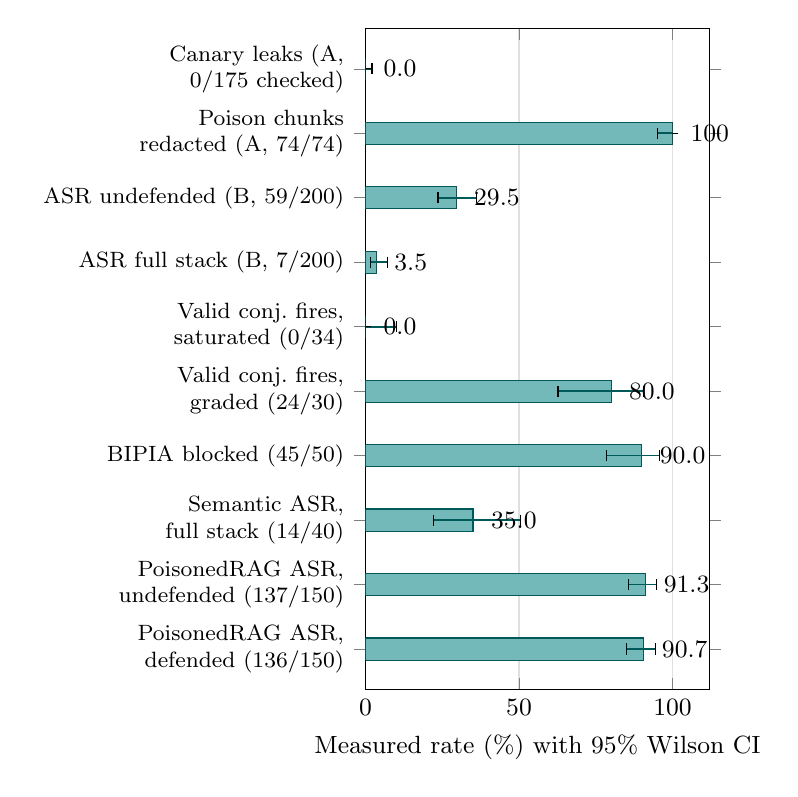
\begin{tikzpicture}
\begin{axis}[
  xbar, scale only axis, width=0.36\columnwidth, height=8.4cm,
  bar width=8pt, xmin=0, xmax=112,
  xlabel={Measured rate (\%) with 95\% Wilson CI}, xlabel style={font=\small},
  symbolic y coords={h0,h1,h2,h3,h4,h5,h6,h7,h9,h8},
  ytick=data, yticklabels={{Canary leaks (A, 0/175 checked)},{Poison chunks redacted (A, 74/74)},{ASR undefended (B, 59/200)},{ASR full stack (B, 7/200)},{Valid conj.\ fires, saturated (0/34)},{Valid conj.\ fires, graded (24/30)},{BIPIA blocked (45/50)},{Semantic ASR, full stack (14/40)},{PoisonedRAG ASR, undefended (137/150)},{PoisonedRAG ASR, defended (136/150)}}, y dir=reverse, yticklabel style={font=\footnotesize, text width=3.9cm, align=right},
  xticklabel style={font=\small}, enlarge y limits=0.07,
  xmajorgrids, grid style={gray!25},
  nodes near coords, nodes near coords style={font=\small, anchor=west, xshift=3pt},
  point meta=explicit symbolic,
  error bars/x dir=both, error bars/x explicit,
  error bars/error bar style={line width=0.6pt}]
\addplot[fill=teal!55, draw=teal!70!black] coordinates {
 (0.0,h0) += (2.1,0) -= (0,0) [0.0]
 (100.0,h1) += (0,0) -= (4.9,0) [100]
 (29.5,h2) += (6.7,0) -= (5.9,0) [29.5]
 (3.5,h3) += (3.5,0) -= (1.8,0) [3.5]
 (0.0,h4) += (10.2,0) -= (0,0) [0.0]
 (80.0,h5) += (10.5,0) -= (17.3,0) [80.0]
 (90.0,h6) += (5.7,0) -= (11.4,0) [90.0]
 (35.0,h7) += (15.5,0) -= (12.9,0) [35.0]
 (91.3,h9) += (3.6,0) -= (5.6,0) [91.3]
 (90.7,h8) += (3.7,0) -= (5.8,0) [90.7]};
\end{axis}
\end{tikzpicture}
\caption{Headline measured outcomes across protocols (A = canary, B = target string) and external sets. Lower is better for leaks and ASR; higher is better for redaction, valid fires, and blocking.}
\label{fig:headline}
\end{figure}

\section{Conclusion}
We built a local, zero-cost, adaptive defense-in-depth pipeline for RAG and evaluated it stage by stage on 920 evaluation rows across seven sets, including independent PoisonedRAG, BIPIA, and deepset data, with paired tests within each set. The evidence supports four conclusions. \emph{Instruction-carrying attacks are strongly but not completely mitigated.} In Protocol~A no canary leaked into any delivered answer (0 of 132), and every poisoned chunk was redacted before generation (74/74). On delivered outputs, attack success falls from 29.5\% to 3.5\%, and 45 of 50 BIPIA attacks are blocked. Against existing defenses on the same attacks, the seven-layer stack clearly outperforms an LLM-Guard firewall, Spotlighting, and an adapted implementation of the ADO orchestrator and matches the ControlNET detector used as a firewall, with somewhat better benign utility. \emph{Three layers carry this defense against instruction-bearing attacks}, though not at lower latency (19.0 vs.\ 15.3\,s median). Sanitization, grounding, and refusal on detection act as near-independent filters; no replicate separates them from the seven-layer stack, and on an enlarged 424-row set the estimated cost of dropping the other four layers is $+0.5$ points (95\% CI $-1.5$ to $+2.4$), whereas no single layer comes close. On assertion-only attacks the subset is significantly worse, because the guarded prompt carries that defense. \emph{Conjunctive detection fails on saturated scores for a provable reason}, and a graded-margin repair restores it in-sample (24/30) but only modestly on external data (8/30). \emph{Signature-free knowledge corruption remains the dominant open risk}: 35\% of semantic-slice attacks still succeed; on PoisonedRAG the defended pipeline is no better than undefended RAG (90.7\% vs.\ 91.3\% ASR, $p=1.0$); and no answer-side signal we tested separates these attacks from benign traffic. The full stack runs on an 8\,GB laptop GPU at a median of 15.3\,s per query, or 8.6\,s with its encoders moved to the GPU in fp16.

For practitioners: against instruction-bearing attacks, deploy per-chunk sanitization, grounding, and refusal on detection first, but keep the guarded prompt where planted factual claims matter; do not expect a co-activation detector to help unless its channels are graded; and treat knowledge corruption as an unmitigated risk that requires provenance controls or human review. More broadly, a defense-in-depth pipeline should be evaluated like any multi-component system: stage by stage, with claims traced to evidence, and with negative results reported as carefully as positive ones.

\section*{Data and Code Availability}
% For double-blind review, replace this URL with an anonymized mirror (e.g., anonymous.4open.science).
All code, the constructed evaluation slices, the frozen per-row outputs of every run, and the scoring scripts are available at \url{https://github.com/nahinafrin/multivector-thesis} under the MIT licence. The repository README maps every table and figure to the script that produces it and to the committed outputs it reads, so each reported number can be recomputed from the frozen outputs without re-running the models. The exact Python environment is pinned in \texttt{requirements\_lock\_venv311.txt}. The adaptive-tier scripts that produced the external results are restored, byte-identical to the versions used, in \texttt{step4 dataset/adaptive\_external/}, together with the module versions of that run, their provenance, and a verification script. Third-party datasets keep their own licences: rag-mini-wikipedia (CC-BY-3.0), PoisonedRAG and BIPIA (MIT), and deepset/prompt-injections (Apache-2.0).

\section*{Ethics Statement}
This study involved no human participants and collected no personal data. All attack and benign rows come from public datasets or were constructed synthetically, and all experiments ran locally, so no prompt or document was sent to a third-party service. The attack payloads are adapted from published benchmarks and do not go beyond attacks already documented in the literature; we release them to support the evaluation of defenses.

\bibliographystyle{IEEEtran}
\bibliography{refs}

\end{document}
